\section{Introduction}

Recommender systems \cite{ricci2011introduction} have become common in a variety of areas including movies, music, videos, news, books, and products in general.
They produce a list of recommended items by either collaborative or content based filtering.
Collaborative filtering methods \cite{amazon-recommender,sarwar01item} build models of the past user-item interactions, while content based filtering \cite{lops2011content} typically generates lists of similar items
based on item properties.

In order to assess the attitude towards the items viewed, recommender systems rely on the feedback provided by the user.
The feedback may be explicit, such as one to five stars ratings of movies in Netflix \cite{adhikari2012unreeling}. 
However, in most of the cases users do not provide like or dislike information, therefore recommenders rely on the implicit feedback such as time elapsed viewing an item or listening to a song.  

The Netflix Prize Challenge \cite{bennett2007netflix,koren2009bellkor} revolutionized our knowledge on recommender systems, however resulted in a bias towards explicit feedback in research.
In most Web services, the users are reluctant to create logins and prefer to browse anonymously.  Or we purchase certain types of goods, for example expensive electronics, so rarely that our previous purchases will be insufficient to create a meaningful user profile.
Several practitioners \cite{koenigstein2013towards} argue that most of the recommendation tasks they face are implicit feedback and without sufficient user history.
In \cite{pilaszy2015neighbor} the authors claim that 99\% of the recommendations systems they built for industrial application tasks are implicit, and most of them are item-to-item. 
In these cases, we have to rely on the recent items viewed by the user in the actual shopping session.

%% Implicit recommendation can be challenging even for frequent items. The problem is even harder if we know little about the particular user who we want to recommend. This kind of ``cold start'' problem could be handled as a

In this paper we consider user independent item-to-item recommendation \cite{sarwar01item,amazon-recommender} especially in case of session recommendation. 
Best known example of this task is the Amazon list of books related to the last visited one \cite{amazon-recommender}. 
To provide the related list, an intuitive approach is to simply considers item pair frequencies.  However, for rare items, it is necessary to use global similarity data to avoid recommendations based on very low support.
In addition, we have to devise techniques that handle new items well. In the so-called cold start case \cite{schein2002methods}, the new items have yet insufficient number of interactions to reliably model their relation to the users.

Our key idea is to utilize the known, recent or popular items for item-to-item recommendation via multiple representations. The starting point of our method is the idea of \cite{koenigstein2013towards} to utilize the entire training data and not just the item-item conditional probabilities.
The authors propose a latent factor model for item-item pairwise relations by a low dimensional embedding. Our main result is a generative model that captures item-to-item interactions by modeling arbitrary item-item distance metrics instead of distance among low dimensional embeddings, which may only use $\ell_2$ or some other vector space norm. 
%Our new idea is to replace the ``black box'' embedding, and model item relations by a generative model defined through a Markov network reflecting the topology of the data set.  
%The main advantage of our method is that we may use item similarity measures 
Our item-to-item model is able to use single or combined similarity measures such as Jaccard or cosine based on collaborative, content, multimedia and metadata information. 

%Also, unlike \cite{koenigstein2013towards} 
% where special tricks are needed to provide nearest neighbor search due to the bias terms in their formulas,
%we develop a full metric space where nearest neighbor data structures can be freely used.

We also consider the top-$n$ recommendation task \cite{deshpande2004item} where for each item we have to provide a sorted list of best next items for the session.
% In this paper, just as in \cite{koenigstein2013towards}, we conducted experiments by adding 200 sampled items to the testing item to evaluate recommendations.

We evaluate our models both by the ``traditional'' top-$n$ recommendation metrics (Recall, DCG) and the recently proposed Mean Percentile Rank (MPR) \cite{hu2008collaborative}.
We observe that the two classes of metrics behave rather differently, however our solution outperforms all baseline methods for infrequent item-to-item recommendation under both circumstances.

Finally, the code used for preprocessing the data sets and experimenting with our method and the baselines is made publicly available.

%  and the data preprocessing steps, including all filtering steps starting from the official data sets at 
% \url{https://github.com/frederickayala/item2item_fisher}.

%https://www.dropbox.com/sh/h84pq66l3sfut5m/AAAR9yiSZnYMG7jbJZnkTq9ya?dl=0}}.

\section{Related work}

Recommender systems are surveyed in \cite{ricci2011introduction}.
A large part of recent recommender systems publications consider the Netflix Prize Competition  \cite{bennett2007netflix}, where ratings were explicitly given (1--5 stars) and the task was to predict unseen ratings.
In this paper, we consider cases where users give no explicit ratings and we have to infer their preferences from their implicit feedback \cite{koenigstein2013towards}.
Even more, we assume that a rich user history is not available as most recommendation tasks in the industry are called item-to-item \cite{pilaszy2015neighbor}. Our model exploits only information available is the present user session.

The first item-to-item recommender methods \cite{sarwar01item,amazon-recommender} were using similarity information to directly find nearest neighbor \cite{desrosiers2011comprehensive} transactions. 
Another solution is to extract association rules \cite{davidson2010youtube}.
Both classes of these methods deteriorate if the last item of the session is rare. That is, it has a low item transition support.

Nearest neighbor methods were criticized for two reasons.  First, the similarity metrics typically have no mathematical justification. Second, the confidence of the similarity values is often not involved when finding the nearest neighbor, which leads to overfitting in sparse cases. 
In \cite{koren2010factor}, a method is given that learns similarity weights for users, however the method gives global and not session based user recommendation.

A new method to give session recommendations was described in \cite{rendle2010factorizing} by Rendle et al.\ that models the users by factorizing personal Markov chains.
Their method is orthogonal to ours in that they provide more accurate user based models if more data is available, while we concentrate on extracting actionable knowledge from the entire data for the sparse transactions in a session.

Closest to our work is Koenigstein and Koren \cite{koenigstein2013towards} with their proposed EIR model.
We use, to the greatest extent reproducible, their experimental settings.
They resolve the sparsity problem by computing latent item factors by using all training data and representing all items in a low dimensional space. Our model is differs in that we do not need to optimize a vector space to learn the transition probabilities in a lower dimensional space. Instead, we start from an arbitrary similarity definition and we may extend similarity for all items, by using all training data, in a mathematically justified way.

% The advantage of our item model is that we are not restricted to vector space metrics when defining the model (the low dimensional embedding, in their case). {\color{red}TODO:\textit{Why are vector space a restriction?}}
% Starting out from an arbitrary similarity definition, we may extend similarity for all items, by using all training data, in a mathematically justified way.

Finally we mention that item-to-item recommendation was also considered as a special context aware recommendation problem.
In \cite{hidasi2012fast} sequentiality as context is handled by using pairwise associations as features in an alternating least squares model by Hidasi et al.
They mention that they face the sparsity problem in setting minimum support, confidence and lift of the associations and they use category of last purchased item as fallback.
In a follow-up result \cite{hidasi2013context}, they use the same context-aware ALS algorithm, however they only consider seasonality as context in that paper.
Our result can be used independently of the ALS based methods and can easily be combined with user personalization. 

The rest of the paper is organized as follows. First we introduce the concept of our generative model, the similarity graph in Section~\ref{sec:sim_graph}. Then, in Section~\ref{sec:fisher} and \ref{sec:fisher_sim} we discuss how the Fisher Information can estimate differentiable probabilities for infrequent items using the similarity graph and we proposed two models, the Item-Item Fisher Conditional Score (FC) and Item-Item Fisher Distance (FD). Finally, we review traditional similarity measures in Section~\ref{sec:sims} and we show our experiments on four real-life data sets in Section~\ref{sec:experiments} focusing on infrequent item-to-item transitions.

\section{Similarity graph}
\label{sec:sim_graph}

We start out with a certain measure of similarity between pairs of items based possibly on implicit or explicit user feedback as well as additional, user independent metadata such as text description, linkage or even multimedia content. 
By the pairwise similarity values and potentially other model parameters $\theta$, we model item $i$ as a random variable $p (i|\theta)$. 
From $p (i|\theta)$, we will infer the distance and the conditional probability of pairs of items $i$ and $j$ taking into account any available implicit, explicit or additional metadata.

Formally, let us consider a certain sample of items $S=\{i_1,i_2,\ldots,i_N\}$ (e.g. most popular or recent items), and assume that we can compute the distance of any item $i$ from each of $i_n \in S$. We will consider our current item $i$ along with its distance from each $i_n\in S$ as a random variable generated by a Markov Random Field (MRF). Random fields are a set of (dependant) random variables. In case of MRF the connection between the elements is described by an undirected graph satisfying the Markov property \cite{besag1975statistical}. For example, the simplest Markov Random Field can be obtained by using a graph with edges between item $i$ and items $i_n\in S$, as shown in  Fig.~\ref{fig:pairwise}. 

\begin{figure}
\centerline{
  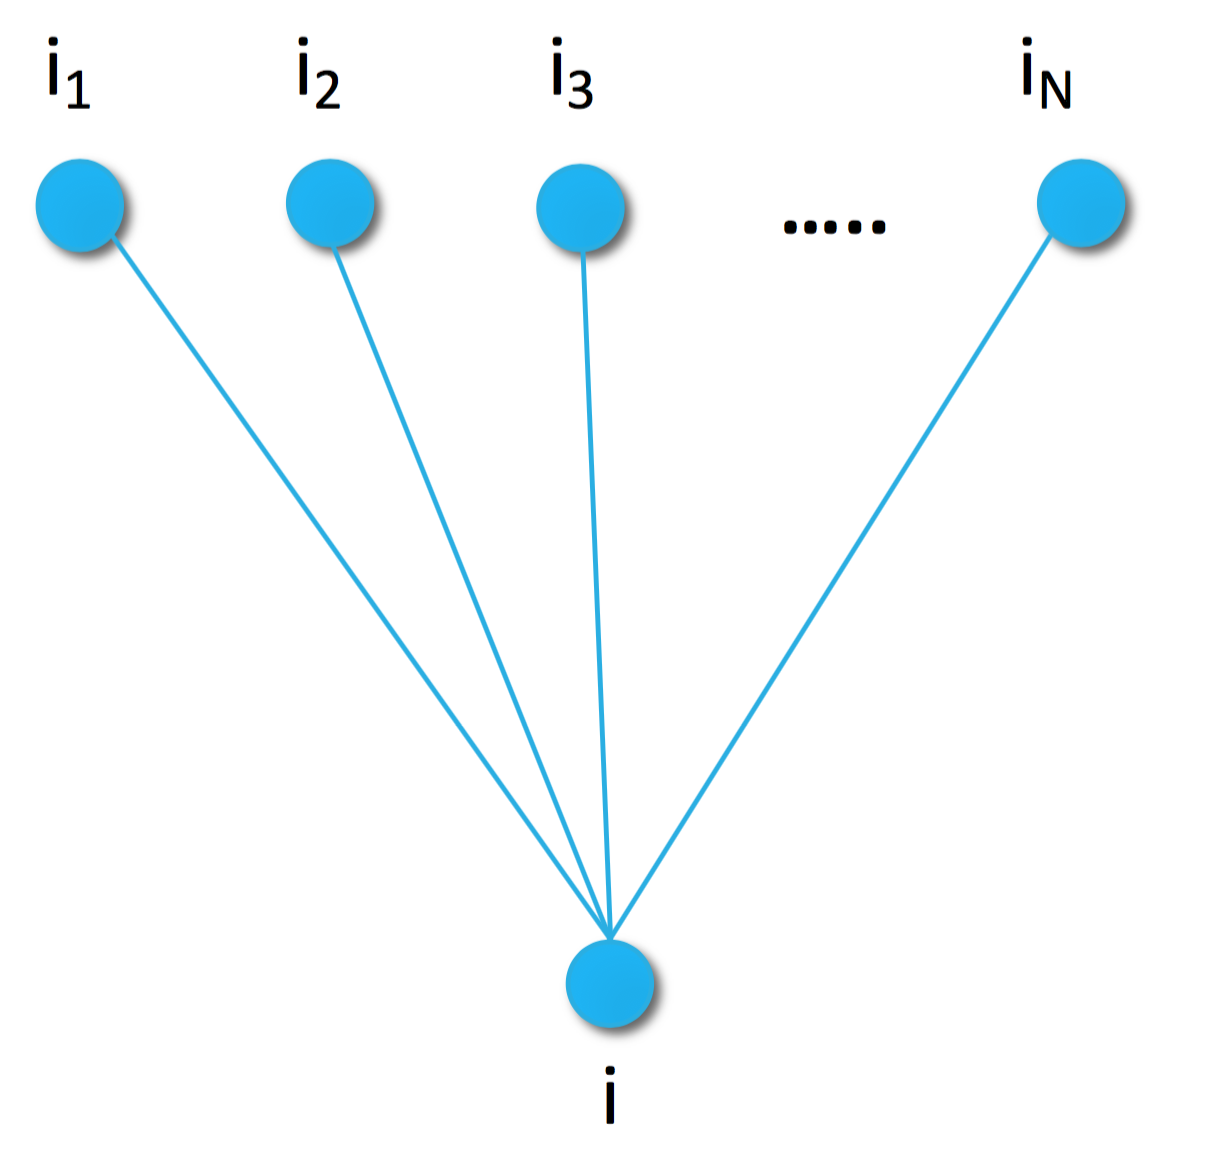
\includegraphics[scale=.2]{i2i_pair.png}}

\caption[]{Similarity graph of item $i$ with sample items $S=\{i_1,i_2,...,i_{N}\}$ of distances $\mbox{dist}(i,i_n)$ from $i$.}
\label{fig:pairwise}
\end{figure}

Let us assume that we are given a Markov Random Field generative model for $p (i|\theta)$.
By the Hammersley-Clifford theorem \cite{hammersley1971markov}, the distribution of $p (i|\theta)$ is then a Gibbs distribution and distribution is factorized over the maximal cliques.
As the theorem states in more detail, given the potential function over the maximal cliques of the random field, the distribution has a form:
%of the generative model for $i$ is a Gibbs distribution of form
%
\begin{equation}
    p(i \mid \theta) = {\mathrm{e}^{-U(i\mid \theta)}}/{Z(\theta)}
    \label{eq:gibbs}
\end{equation}
%
where $U(i\mid \theta)$ is the energy function and 
%
\begin{equation}
Z(\theta) = \sum_{i} \mathrm{e}^{-U(i \mid \theta)}
\nonumber
\end{equation}
%
is the sum of the exponent of the energy function over our generative model, a normalization term called the partition function. If the model parameters are previously determined, then $Z(\theta)$ is a constant. 

Given a Markov Random Field defined by a certain graph such as the one in Fig.~\ref{fig:pairwise} (or some more complex graph defined later), a wide variety of proper energy functions can be used to define a Gibbs distribution. The weak but necessary restrictions are that the energy function has to be positive real valued, additive over the maximal cliques of the graph, and more probable configurations (specific sets of parameters) have to have lower energy. 

Now we define the simplest similarity graph seen in Fig.~\ref{fig:pairwise} as follows. Let be a finite sample set $S=\{i_1,..,i_{N}\}$ and a distance (or divergence) defined over any item pairs be given.  Since all the edges are between the elements of the sample set and the particular item $i$, we may formulate the energy function for \eqref{eq:gibbs} as
%
\begin{equation}
U(i \mid \theta=\{\alpha_1,..,\alpha_{N}\}) := \sum_{n=1}^{N} \alpha_n \mbox{dist}(i,i_n),
\label{eq:potential}
\end{equation}
 %
where $\theta$ is the hyperparameter set defined over the elements in the sample set. 


\begin{figure}
\centerline{
  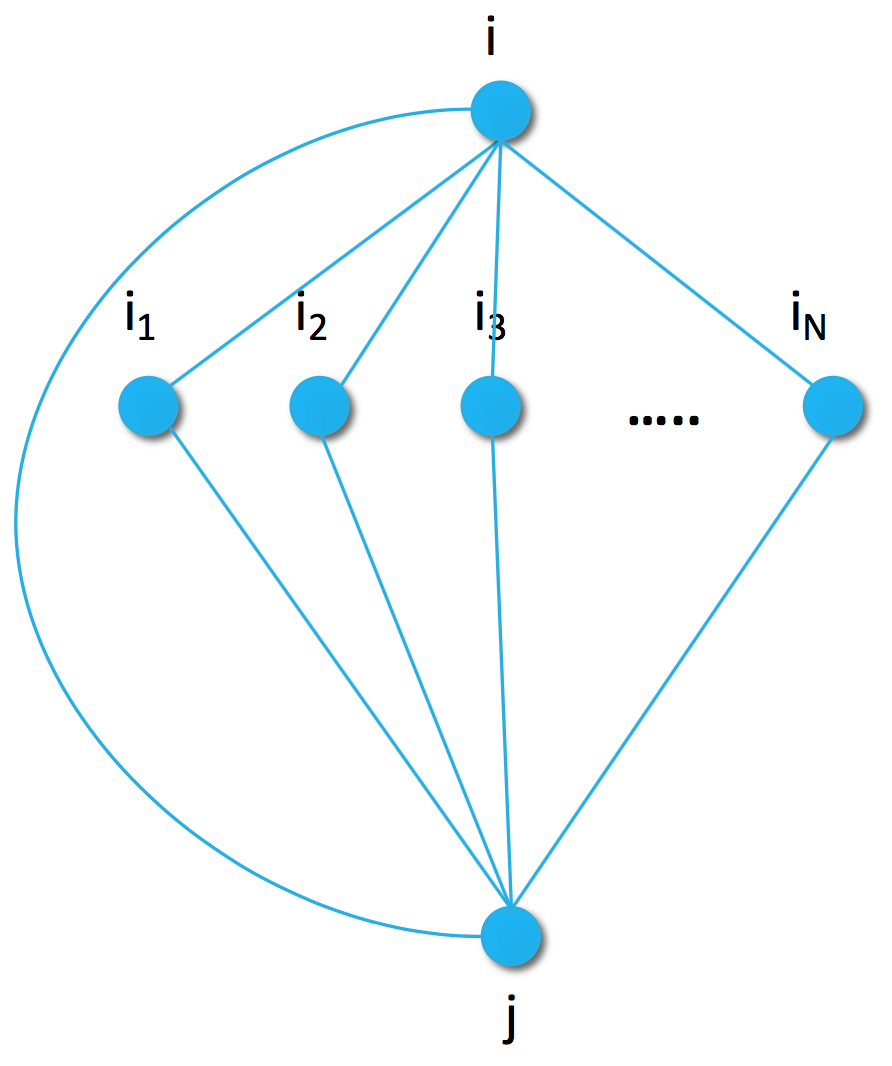
\includegraphics[scale=.2]{i2i_joined.png}}

\caption[]{Pairwise similarity graph with sample set $S=\{i_1,i_2,...,i_{N}\}$ for a pair of items $i$ and $j$.}
\label{fig:join}
\end{figure}


In a more complex model, we capture the connection between pairs of items by extending the generative graph model with an additional node for the previous item as shown in Fig.~\ref{fig:join}.  In the pairwise similarity graph, the maximal clique size increases to three. To capture the joint energy, we can use a heuristic approximation similar to the pseudo-likelihood method \cite{besag1975statistical}, thus we approximate the joint distribution of each size three clique as the sum of the individual edges, as follows:
%
\begin{equation}
\label{eq:potential_joined}
U(i,j \mid \theta) := \sum_{n=1}^{N} \beta_{n} (\mbox{dist}(i,i_n) + \mbox{dist}(j,i_n) + \mbox{dist}(i,j)),
\end{equation}
%
where $\theta = \{\beta_n\}$.

At first glance, the additive approximation seems to oversimplify the clique potential and falls back to the form of equation \eqref{eq:potential}. However, the effect of the clique is apparently captured by the common clique hyperparameter $\beta_{n}$, as also confirmed by our experimental results. 

\section{Fisher Information}
\label{sec:fisher}

Items with low item support usually are not differentiable using traditional similarity models. That is, the similarity score is equal for the items. To overcome this, we use the Fisher information to estimate differentiable probabilities even for rare items given the previously introduced similarity graphs by taking advantage of the invariance properties of the Fisher metric.

Let us consider a general parametric class of probability models $p(i| \theta)$, where $\theta\in \Theta \subseteq \mathbb{R}^\ell$ lies in a space 
% as defined for example by the similarity graphs of equation~\eqref{eq:gibbs}, 
of some positive integer dimension $\ell$. The collection of models with parameters from a general hyperparameter space $\Theta$ can then be viewed as a (statistical) manifold $M_\Theta$, provided that the dependence of the potential on $\Theta$ is sufficiently smooth. By \cite{Jo}, $M_\Theta$ can be turned into a Riemann manifold by giving an inner product (kernel) at the tangent space of each point $p(i| \theta) \in M_\Theta$, where the inner product varies smoothly with $p$. 

The notion of the inner product over $p(i| \theta)$ allows us to define the so-called Fisher metric on $M$. The fundamental result of \u{C}encov \cite{cencov1982} states that the Fisher metric exhibits a unique invariance property under some maps which are quite natural in the context of probability. Thus, one can view the use of Fisher kernel as an attempt to introduce a natural comparison of the items on the basis of the generative model \cite{JH}. 

We start defining the Fisher kernel over the manifold $M_\Theta$ of probabilities $p(i| \theta)$ as in equation~\eqref{eq:gibbs} by considering the tangent space.
The tangent vector 
\begin{equation}
G_i=\nabla_\theta \log p(i|\theta)=\left(
\frac{\partial}{\partial \theta_1} \log p(i|\theta), \ldots,
\frac{\partial}{\partial \theta_l} \log p(i|\theta)\right)
\label{eq:Fisher-score}
\end{equation}
is called the {\em Fisher score} of item $i$. 
The {\em Fisher information matrix} is a positive semidefinite matrix defined as
%
\begin{equation}
F(\theta):= {\bf E_{\theta}}(\nabla _\theta\log p(i|\theta)\nabla _\theta \log p(i|\theta)^T),
\label{eq:fi}
\end{equation}
%
%Now the mapping $i\mapsto \phi_i $ of items to feature vectors can be $i\mapsto F^{-\frac 12}G_i$ (we suppressed here the dependence on $\theta$), the {\em Fisher vector} where $F(\theta)$ is a positive semidefinite matrix, which varies smoothly with the base point $\theta$. Such positive semidefinite matrices are provided by the Fisher information matrix
%
%
where the expectation is taken over $p(i|\theta)$. In particular, the $nm$-th entry of 
$F(\theta)$  is 
$$ F_{nm}=\sum_{i} p(i|\theta)
\left(\frac{\partial}{\partial \theta_n} \log p(i|\theta)\right)
\left(\frac{\partial}{\partial \theta_m} \log p(i|\theta)\right).$$

Thus, to capture the generative process, the gradient space of $M_\Theta$ is used to derive the Fisher vector, a mathematically grounded feature representation of item $i$. The corresponding kernel function 
%
\begin{equation}
K(i,j):= G^T_iF^{-1}G_j
\label{eq:Fisher-kernel}
\end{equation}
%
is called the {\em Fisher kernel}. An intuitive interpretation is that $G_i$ gives the direction where the parameter vector $\theta$ should be changed to fit item $i$ the best \cite{perronnin2007fisher}. In addition, we prove a theorem for our kernels on a crucial reparametrization invariance property that typically holds for Fisher kernels \cite{janke2004information}. 
%\newtheorem{theorem}{Theorem}
\begin{theorem}
For all $\theta = \rho(\mu)$ for a continuously differentiable function $\rho$, $K_\theta$ is identical.
\end{theorem}
%
\begin{proof}
The Fisher score is
\begin{equation}
G_i(\mu) = G_i(\rho(\mu)) \bigg(\frac {\partial\rho}{\partial \mu}\bigg) 
\end{equation}
%
and therefore 
%
\begin{gather*}
K_{\mu}(i,j) = G_i(\mu) F_{\mu}^{-1} G_j(\mu) \\ 
= G_i(\rho(\mu)) \bigg(\frac {\partial\rho}{\partial \mu}\bigg) \Bigg(F_{\rho(\mu)} \bigg(\frac {\partial\rho}{\partial \mu}\bigg)^2 \Bigg)^{-1} G_j(\rho(\mu))\bigg(\frac {\partial\rho}{\partial \mu}\bigg) \\
= G_i(\rho(\mu)) F_{\rho(\mu)}^{-1}  G_j(\rho(\mu)) = K_{\rho}(i,j).
\square
\end{gather*}
%\end{gather*}
\end{proof} 

Essentially, the theorem states that the kernel will not depend on the hyperparameters $\theta$.

\section{Item Similarity by Fisher information}
\label{sec:fisher_sim}

Fisher information has been used in fields like DNA splice site classification \cite{JH} or computer vision \cite{perronnin2007fisher} but not in recommender systems. Based on the similarity graphs introduced in Section~\ref{sec:sim_graph} and by taking advantage of the invariance properties of the Fisher metric we propose two ranking methods for item-item transitions.
 
\subsection{Item-Item Fisher Conditional Score (FC)}
\label{sec:fs_rank}
\label{sect:FC}

Our first item-to-item recommender method will involve similarity information in the item-item transition conditional probability computation by using Fisher scores as in equation~\eqref{eq:Fisher-score}.
By the Bayes theorem,
%
\begin{equation*}
G_{j|i} = \nabla_{\theta} \log p(j \mid i; \theta) = \nabla_{\theta} \log \frac{p(i,j \mid \theta)}{p(i \mid \theta)}
\nonumber
\end{equation*}
%
\begin{equation}
= \nabla_{\theta} \log p(i,j \mid \theta) - \nabla_{\theta} \log p(i \mid \theta),
\label{eq:fisher_score_cond}
\end{equation}
%
thus we need to determine the joint and the marginal distributions for a particular item pair. 

First, let us calculate the Fisher score of \eqref{eq:Fisher-score} with $p (i|\theta)$ of the single item generative model defined by \eqref{eq:potential}, 
%
\begin{equation}
\begin{split}
    G_i^k(\theta) &=\nabla_{\theta_k} \log p(i|\theta)\\
          &= \frac{1}{Z(\theta)}\sum_{i} \mathrm{e}^{-U(i \mid \theta)} \frac{\partial{U(i \mid \theta)}}{\partial{\theta_k}} - \frac{\partial{U(i \mid \theta)}}{\partial{\theta_k}} \\
          &= \sum_{i} \frac{\mathrm{e}^{-U(i \mid \theta)}}{Z(\theta)} \frac{\partial{U(i \mid \theta)}}{\partial{\theta_k}} - \frac{\partial{U(i \mid \theta)}}{\partial{\theta_k}}.
\end{split}
\nonumber
\end{equation}
%
By \eqref{eq:gibbs}, our formula can be simplified as 
%
\begin{equation}
\begin{split}
    G_i^k(\theta) &= \sum_{i} p(i \mid \theta) \frac{\partial{U(i \mid \theta)}}{\partial{\theta_k}} - \frac{\partial{U(i \mid \theta)}}{\partial{\theta_k}} \\
    				 &= {\textstyle {\bf E_{\theta}}[\frac{\partial{(U(i \mid \theta)}}{\partial{\theta_k}}] - \frac{\partial{U(i \mid \theta)}}{\partial{\theta_k}}.}
\end{split}
\label{eq:gix}
\end{equation}
%
For an energy function as in equation \eqref{eq:potential}, the Fisher score of $i$ has a simple form,
%
\begin{equation}
    G_i^k(\theta)= {\bf E_{\theta}}[\mbox{dist}(i,i_k)] - \mbox{dist}(i,i_k),
\label{eq:fisher_pair}
\end{equation} 
%
and similarly for equation \eqref{eq:potential_joined}, 
%
\begin{equation}
\begin{split}
    G_{ij}^{k}(\theta) = {\bf E_{\theta}}[\mbox{dist}(i,i_k) + \mbox{dist}(j,i_k)+\mbox{dist}(i,j)] \\
    - (\mbox{dist}(i,i_k)+ \mbox{dist}(j,i_k)+\mbox{dist}(i,j)). 
\end{split}
\label{eq:fisher_joined}
\end{equation} 

Now, if we put \eqref{eq:fisher_pair} and \eqref{eq:fisher_joined} into \eqref{eq:fisher_score_cond}, several terms cancel out and the Fisher score has the simple form
%
\begin{equation}
G_{j|i}^k = {\bf E_{\theta}}[\mbox{dist}(j,i_k) + \mbox{dist}(i,j)] - (\mbox{dist}(j,i_k) + \mbox{dist}(i,j)).
\nonumber
\end{equation}
The above formula involves the distance values on the right side, which are readily available, and the expected values on the left side, which may be estimated by using the training data. We note that here we make a heuristic approximation: instead of computing the expected values e.g.\ by simulation, we substitute the mean of the distances from the training data.

As we discussed previously, the Fisher score resembles how well the model can fit the data, thus we can recommend the best fitting next item $j^{*}$ based on the norm of the Fisher score,
%
\begin{equation}
j^{*} = \argmin_{j \neq i} || G_{j|i}(\theta) ||,
\nonumber
\end{equation}
%
where we will use $\ell_2$ for norm in our experiments.

\subsection{Item-Item Fisher Distance (FD)}
\label{sect:FD}

In our second model, we rank the next item by its distance from the last one, based on the Fisher metric. With the Fisher kernel $K(i,j)$, the \emph{Fisher distance} can be formulated as
\begin{equation}
\mbox{dist}_F(i,j) = \sqrt{K(i,i) - 2 K(i,j) + K(j,j)},
\label{eq:Fisher-dist}
\end{equation}   
%
thus we need to compute the Fisher kernel over our generative model as in \eqref{eq:Fisher-kernel}.  The computational complexity of the Fisher information matrix estimated on the training set is $\mathcal{O}(T |\theta|^2)$, where $T$ is the size of the training set.  To reduce the complexity to $\mathcal{O}(T |\theta|)$, we can approximate the Fisher information matrix with the diagonal as suggested in \cite{JH,perronnin2007fisher}.
Hence we will only use the diagonal of the Fisher information matrix, 
%
\begin{equation}
\begin{split}
    F_{k,k} &={\bf E_{\theta}}[\nabla_{\theta_k} \log p(i|\theta)^T \nabla_{\theta_k} \log p(i|\theta)] \\
    &={\bf E_{\theta}}[({\bf E_{\theta}}[\frac{\partial{U(i \mid \theta)}}{\partial{\theta_k}}] - \frac{\partial{(U(i \mid \theta)}}{\partial{\theta_k}})^2] . \\
\end{split}
\nonumber
\end{equation}

For the energy functions of equations \eqref{eq:potential} and \eqref{eq:potential_joined}, the diagonal of the Fisher kernel is the standard deviation of the distances from the samples. We give the Fisher vector of $i$ for 
\eqref{eq:potential}:
%
\begin{equation}
\begin{split}    
    \mathcal{G}_i^k &= F^{-\frac 12} G_i^k \approx F_{kk}^{-\frac 12} G_i^k\\
    &=\frac {{\bf E_{\theta}}[\mbox{dist}(i,i_k)] - \mbox{dist}(i,i_k)} {{\bf E_{\theta}^{\frac 12}}[({\bf E_{\theta}}[\mbox{dist}(i,i_k)] - \mbox{dist}(i,i_k))^2]}.
    \nonumber
\end{split}
\label{eq:kernel}
\end{equation}

The final kernel function is
%
\begin{equation}
\begin{split}
K(i,j) &= G_i^T F^{-1} G_j \approx G_i^T F_{diag}^{-1} G_j \\
	   &= G_i^T F_{diag}^{-\frac 12} F_{diag}^{-\frac 12} G_j = \sum_k \mathcal{G}_i^k \mathcal{G}_j^k.
\end{split}
\nonumber
\end{equation}
By substituting into \eqref{eq:Fisher-dist}, the recommended next item after item $i$ will be
%
\begin{equation}
j^{*} = \argmin_{j \neq i} \text{dist}_F(i,j).
\nonumber 
\end{equation}

\subsection{Multimodal Fisher score and distance}
\label{sec:fish_comb}

So far we considered only a single distance or divergence measure over the items. We may expand the model with additional distances with a simple modification to the graph of Fig.~\ref{fig:pairwise}. 
We expand the points of the original graph into new points $R_i=\{r_{i,1},..,r_{i,|R|}\}$ corresponding to $R$ representatives for each item $i_n$ in Fig.~\ref{fig:multi}. There will be an edge between two item representations $r_{i,\ell}$ and $r_{j,k}$ if they are the same type of representation ($\ell=k$) and the two item was connected in the original graph. This transformation does not affect the maximal clique size and therefore the energy function is a simple addition, as
%
\begin{equation}
U(i \mid \theta) = \sum_{n=1}^{N} \sum_{r=1}^{|R|} \alpha_{nr} \mbox{dist}_r(i_r,i_{nr}),
\label{eq:potential_multi}
\end{equation}
% 
and if we expand the joint similarity graph to a multimodal graph, the energy function will be
%
\begin{equation}
\begin{split}
\label{eq:potential_joined_multi}
U(i,j \mid \theta) = \sum_{n=1}^{N} \sum_{r=1}^{|R|} \beta_{nr} (\mbox{dist}_r(i_r,i_{nr}) \\
+ \mbox{dist}_r(j_r,i_{nr}) + \mbox{dist}_r(i_r,j_r)).
\end{split}
\end{equation}

\begin{figure}
\centerline{
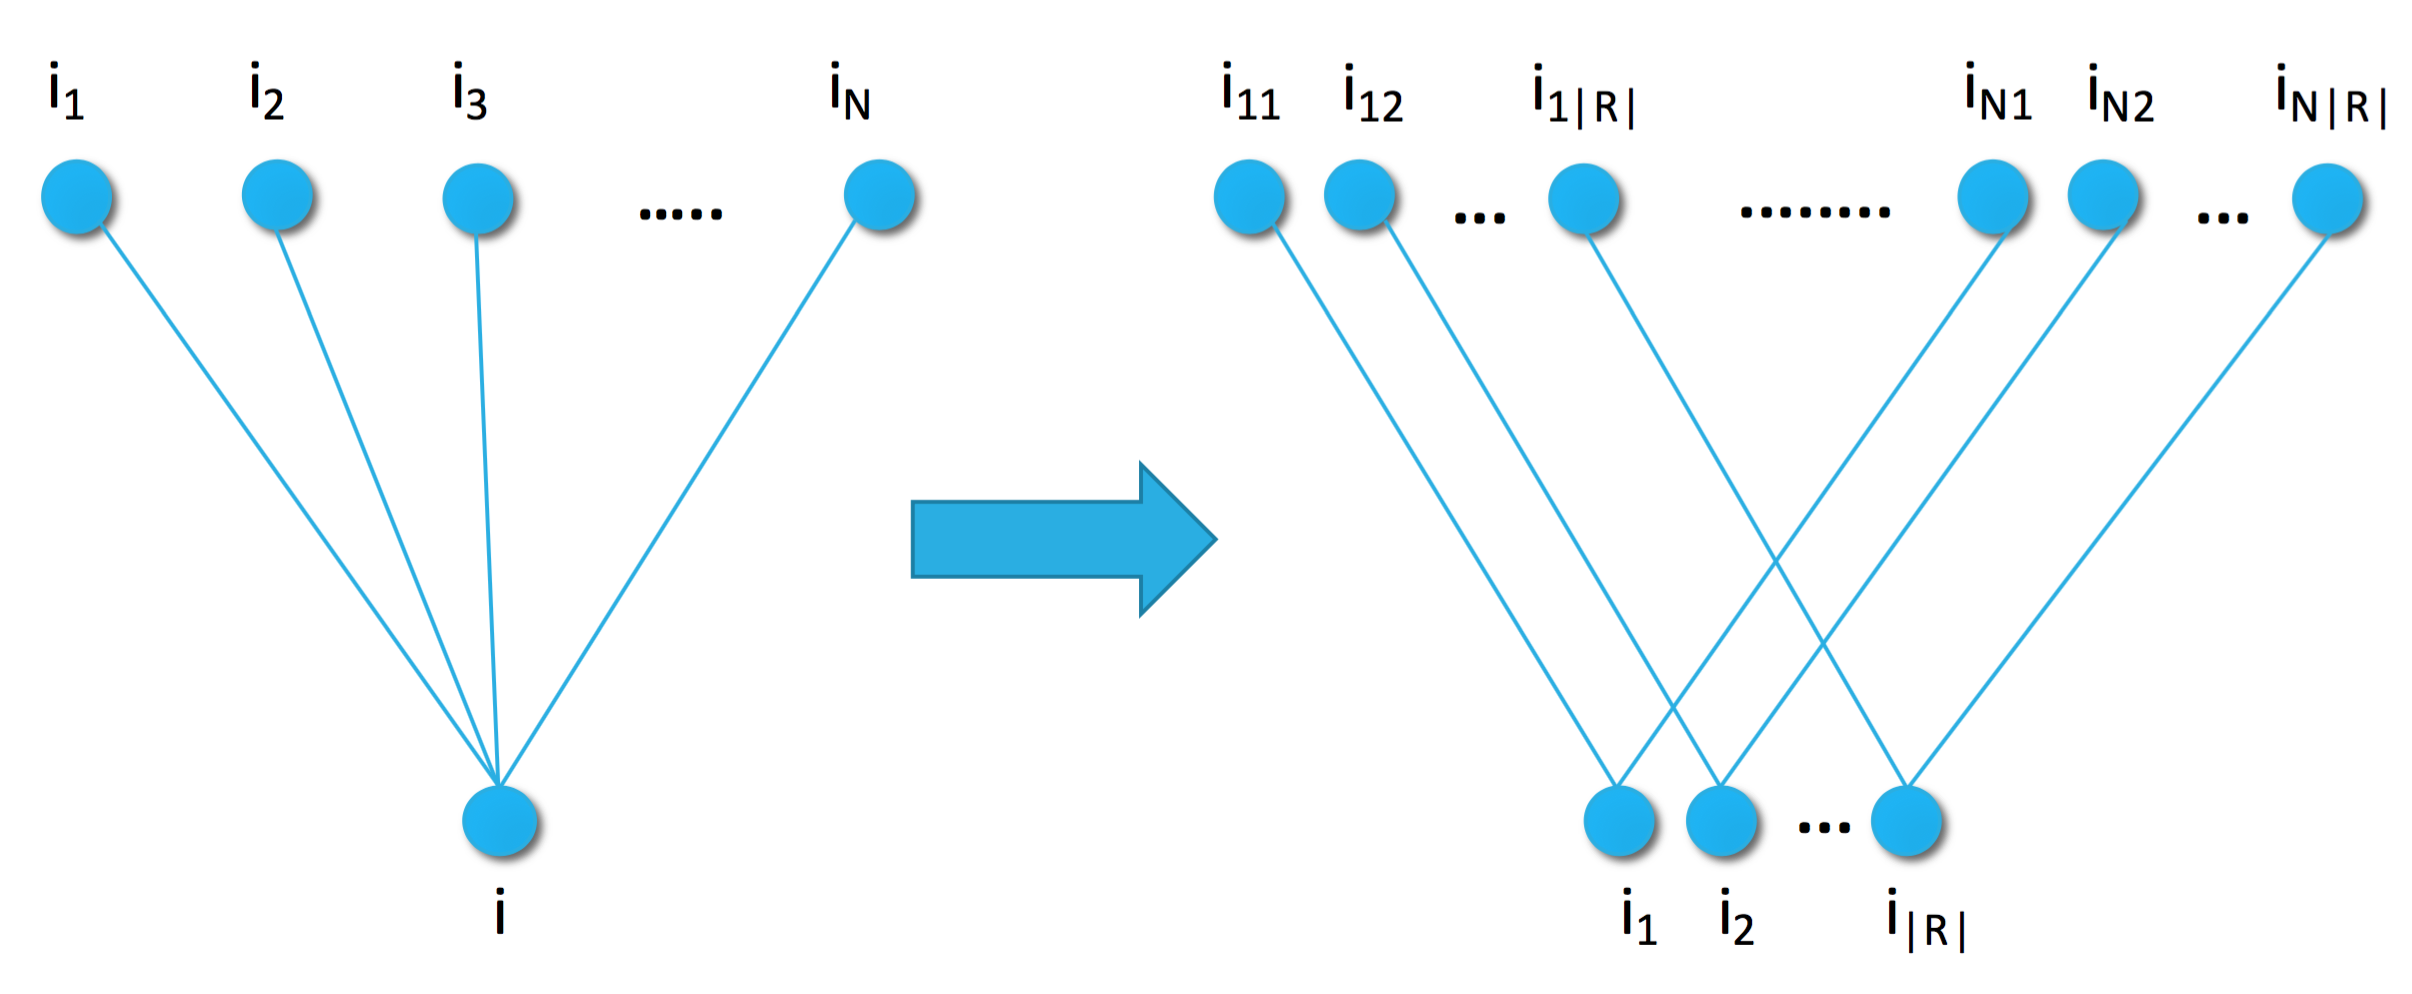
\includegraphics[scale=.2]{i2i_multi.png}}
\caption{The single and multimodal similarity graph with sample set $S=\{i_1,i_2,...,i_{N}\}$ and $|R|$ modalities.}
\label{fig:multi}
\end{figure}

Now, let the Fisher score for any distance measure $r \in R$ be $G_{ir}$, than the Fisher score for the multimodal graph is concatenation of the unimodal Fisher scores as
%
\begin{equation}
G_i^{multi} = \{G_{i1},..,G_{i|R|}\},
\nonumber
\end{equation}
%
and therefore the norm of the multimodal Fisher score is a simple sum over the norms: 
%
\begin{equation}
|| G_i^{multi}|| = \sum_{r=1}^{|R|} ||G_{ir}||.
\label{eq:fs_multi}
\end{equation}
%
The calculation is similar for the Fisher kernel of equation \eqref{eq:kernel}, thus the multimodal kernel can be expressed as
%
\begin{equation}
K_{multi}(i,j) = \sum_{r=1}^{|R|} K_r(i,j).
\label{eq:fk_multi}
\end{equation}

\section{Similarity Measures}
\label{sec:sims}
Next we enumerate distance and divergence measures that can be used in the energy functions \eqref{eq:potential} and \eqref{eq:potential_joined}. 
Without using the Fisher information machinery, these measures yield the natural baseline methods for item-to-item recommendation.
We list both implicit feedback collaborative filtering and content based measures.

\subsection{Feedback Similarity}

For user implicit feedback on item pairs, various joint and conditional distribution measures can be defined based on the frequency $f_i$ and $f_{ij}$ of items $i$ and item pairs $i,j$, as follows.
%
\begin{enumerate}
%
\item Cosine similarity (Cos):
%
\begin{equation}
cos(i,j) = \frac{f_{ij}}{\sqrt{f_i f_j}}.
\nonumber
\end{equation}
%
\item Jaccard similarity (JC):
%
\begin{equation}
JC(i,j) = \frac{f_{ij}}{f_i+f_j-f_{ij}}.
\nonumber
\end{equation}
%
\item Empirical Conditional Probability (ECP): estimates the item transition probability:
%
\begin{equation}
ECP(j|i) = \frac{f_{ij}}{f_i+1},
\nonumber 
\end{equation}
%
where the value 1 is a smoothing constant. 
\end{enumerate}
%
Additionally, in \cite{koenigstein2013towards} the authors suggested a model, the Euclidean Item Recommender (EIR) to approximate the transition probabilities with the following conditional probability
%
\begin{equation}
p(j | i) = \frac{\exp^{-||x_i-x_j||^2 + b_j}}{\sum \exp^{-||x_i-x_k||^2+b_k}},
\nonumber
\end{equation}
%
where they learn a latent vector $x_i$ and bias $b_i$ for item $i$. 

All of the above measures can be used in the energy function as the distance measure after small modifications. 

Now, let us assume that our similarity graph (Fig.~\ref{fig:pairwise}) has only one sample element $i$ and the conditional item is also $i$. The Fisher kernel will be,
%
\begin{equation}
\nonumber
\begin{split}
K(i,j) &= \frac{1}{\sigma_{i}^2} (\mu_i - \mbox{dist}(i,i))(\mu_i-\mbox{dist}(i,j)) \\
       &= \frac{\mu_i^2}{\sigma_{i}^2} - \frac{\mu_i}{\sigma_{i}^2} \mbox{dist}(i,j)) \\
       &= C_1-C_2*\mbox{dist}(i,j),
\end{split}
\end{equation}

where $\mu_i$ and $\sigma_i$ are the expected value and variance of distance from item $i$. Therefore if we fix $\theta$, $C_1$ and $C_2$ are positive constants and the minimum of the 
Fisher distance will be %???

\begin{equation}
\nonumber
\begin{split}
\min_{j \neq i} \text{dist}_F(i,j) &= \min_{j \neq i} \sqrt{K(i,i) - 2 K(i,j) + K(j,j)} \\
                   &= \min_{j \neq i} \sqrt{2C_2*\mbox{dist}(i,j)} = \min_{j \neq i} \mbox{dist}(i,j).
\end{split}
\end{equation}

Hence if we measure the distance over the latent factors of EIR, the recommended items will be the same as defined by EIR (equation~10 in \cite{koenigstein2013towards}).

\subsection{Content Similarity}

We may use item metadata for measuring similarity based on content.
For example, we may use the semantic structure of the items based on DBPedia\footnote{\url{http://wiki.dbpedia.org}} \cite{auer2007dbpedia} by collecting the 
Resource Description Framework (RDF) nodes and links or other semantic knowledge graphs corresponding to the items to be recommended.  % ???
In case of movies, for example, the extracted graph is an entity tree including directors, actors, genre, topics, etc. We have multiple options to define  similarity based on the semantic graph.
We may use the Jaccard similarity or the Jensen-Shannon divergence of the bag of nodes in the semantic graph, or even use Graph kernels \cite{losch2012graph}.

%Let $P$ and $Q$ be the probability distributions for item $i$ and $j$, then the Jensen-Shannon divergence is
%
%\begin{equation}
%\nonumber
%JS(P,Q) = \frac{1}{2} (KL(P||M)+KL(Q||M))
%\end{equation}
%
%where $M=\frac{1}{2}(P+Q)$ and $KL(P||Q)=\sum_i P_i \log \frac{P_i}{Q_i}$ is the Kullback-Leibler divergence. 

\section{Experiments}
\label{sec:experiments}

We performed experiments on four publicly available data sets.
As baseline methods, we computed four item-item similarity measures: Empirical Conditional Probability (ECP), Cosine 
(Cos), Jaccard (JC) as defined in Section~\ref{sec:sims}, 
and we also implemented the Euclidean Item Recommender of \cite{koenigstein2013towards}. 
As content similarity we computed Jaccard similarity. % and Jensen-Shannon divergence. % ??? for content-based recommendation ?
For evaluation, we use Mean Percentile Rank (MPR) \cite{koenigstein2013towards}, Recall, and Discounted Cumulative Gain (DCG), which we define next.

In this paper, just as in \cite{koenigstein2013towards}, we conducted experiments by adding 200 sampled items to the testing item to evaluate recommendations. That is, given the current item in a session $i$ and a known co-occurrence $j$ we add randomly 200 items and rank them based on the score of the models. The best models should preserve $j$ on the top of the sorted list.

\subsection{Evaluation Metrics}

Let us consider an item $i$ and a ranking $r_1,r_2,\ldots$ of the possible next items.
We define Recall@K as a binary value: if the actual next item $j$ is ranked K or higher, Recall@K is one, otherwise zero:
%
\begin{equation}
\mbox{Recall@}K(r_1,\ldots,r_K) = \sum_{\ell=1}^K \delta_{r_\ell,j},
\nonumber
\end{equation}
where $\delta_{r_\ell,j}$ is the Kronecker delta: one if $r_\ell=j$ and zero otherwise. Similarly, DCG@K is defined to be zero if the test 
item j is not in the top K recommended items, otherwise
\begin{equation}
\mbox{DCG@}K(r_1,\ldots,r_K) = \sum_{\ell=1}^K \frac{\delta_{r_\ell,j}}{\log_2(\ell+1)}.
\nonumber
\end{equation} 

%Worth to mention, the presentation of the recommended items may effect the performance.

In \cite{koenigstein2013towards}, the authors measure item-to-item recommendation by mean percentile rank (MPR) as defined next.
Given the ranked list $r_1,r_2,\ldots$ and the actual next item $j$ of rank $k$, $j=r_k$, percentile rank is defined as %???  or -> of cahnged by Adri
%
\begin{equation}
\text{PR}(j) = \sum_{\ell > k} f_\ell / \sum_\ell f_\ell.
\nonumber
\end{equation}
If certain elements are ranked in tie with $j$ we define the percentile rank as
\begin{equation}
\text{PR}(j) = \frac{\sum_{\text{$\ell$ ranked strictly after $j$}} f_\ell + 0.5*\sum_{\text{$\ell$ ranked in tie with $j$}} f_\ell} {\sum_\ell f_\ell}.
\nonumber
\end{equation}
%
Finally, MPR is the mean PR over all testing events.
Unlike Recall and DCG where higher value indicates better performance, for MPR, the lower the better.

The main difference of MPR compared to DCG and Recall is that MPR also takes the  popularity of the items into consideration.
Since the occurrence of the items is typically non-uniform, if a popular item surpasses the actual next item, the penalty in PR could be high.
On the other hand, DCG and Recall give more emphasis to the accuracy of the top recommended items.
As we will see in the experiments, the relation of Recall or DCG with MPR depends on the distribution of the conditional items. 

\subsection{Data sets and Experimental Settings}

We carried out experiments over four data sets: Netflix \cite{bennett2007netflix}, MovieLens\footnote{\url{http://grouplens.org/datasets/movielens/}}, 
Books \cite{ziegler2005improving} and Yahoo!\ Music \cite{dror2012yahoo}. 

Just as in \cite{koenigstein2013towards} we generate the item transitions by creating pairs from the items consumed by the users in the data set. For example, if a user consumed items $a$, $b$ and $c$ we create three co-occurrence pairs. That is, $[(a,b), (b,c), (c,a)]$. We do this for all the users and then we calculate the frequency of each pair. Figure~\ref{fig:kde_occurrence} and Table~\ref{tab:datasets_quartiles} shows that most of the co-occurrence in the datasets are infrequent. 75\% of the pairs have low item support. Because our research is focused on infrequent items, we filtered out the items with high support. The maximum co-occurrence frequency that we considered for the data sets in our experiments are 2 for Books, 23 for Yahoo! Music, 300 for MovieLens and 1241 for Netflix.

\begin{table}[t]
\caption[]{Co-occurrence quartiles}
\centerline{
\begin{tabular}{lrrrr}\hline
\toprule
      Dataset &  25\% &  50\% &   75\% &     Max \\
\midrule
        Books &    1 &    1 &     2 &   1,931 \\
 Yahoo! Music &    4 &    9 &    23 & 160,514 \\
    MovieLens &   29 &  107 &   300 &   2,941 \\
      Netflix &   56 &  217 & 1,241 & 144,817 \\
\bottomrule
\end{tabular}
}
\label{tab:datasets_quartiles}
\end{table}

\begin{figure}
\hfill
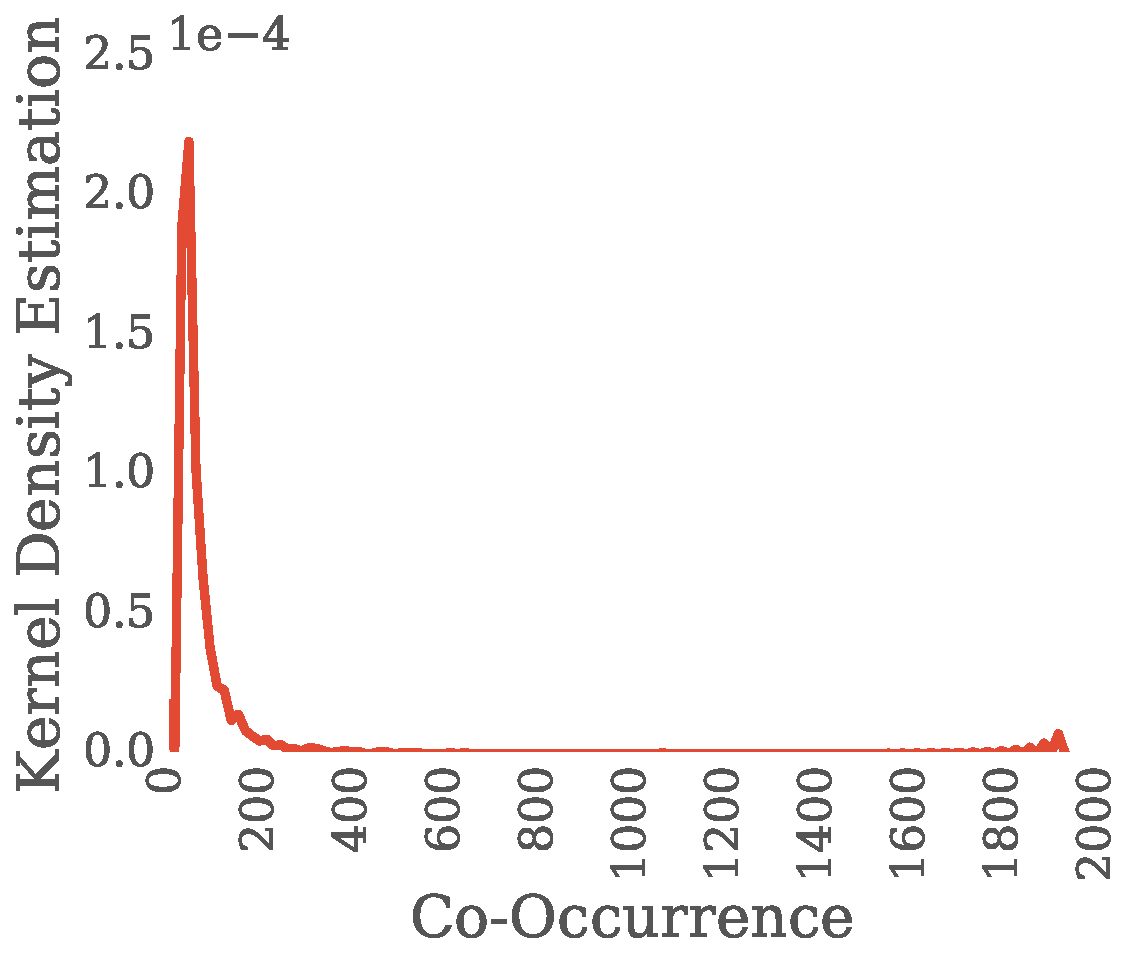
\includegraphics[width=0.23\textwidth]{kde_occurrencebooks.pdf}~%
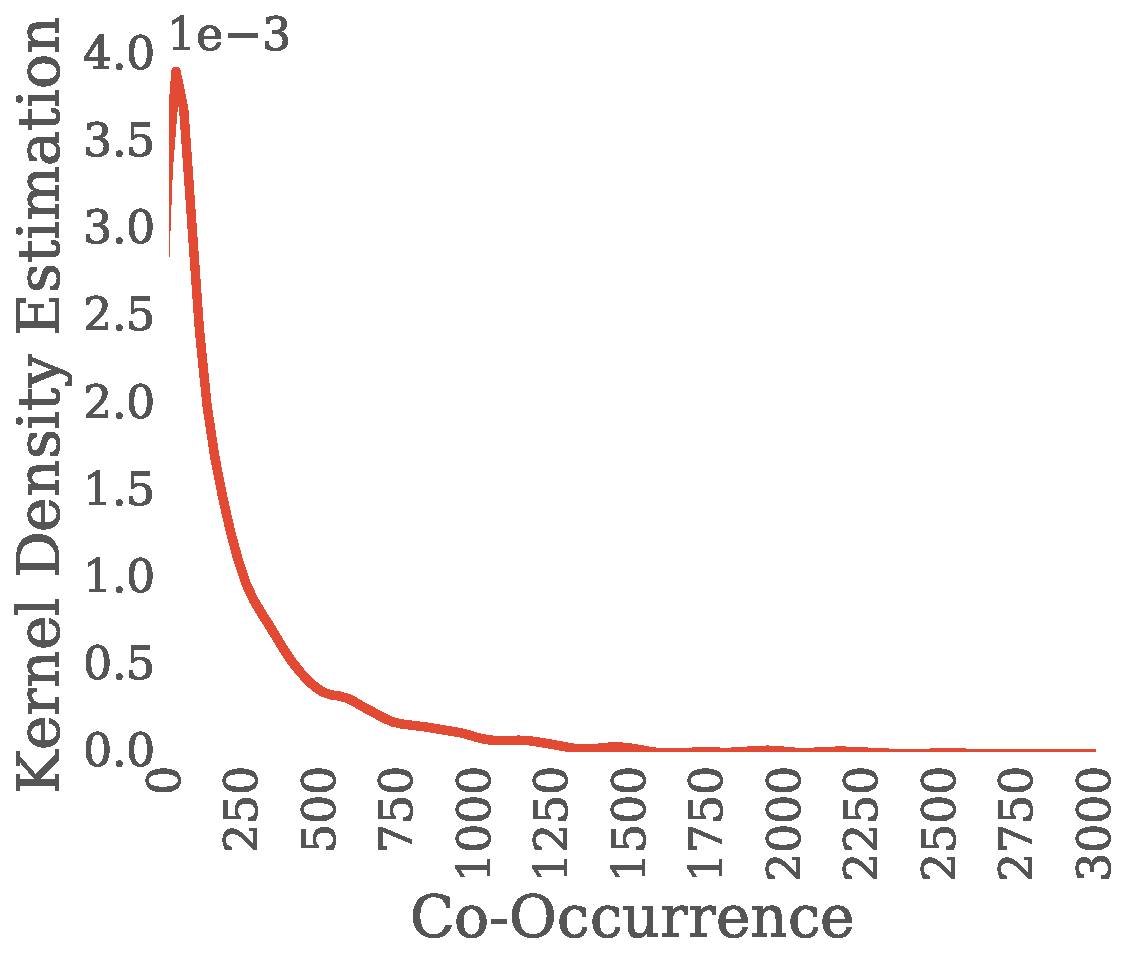
\includegraphics[width=0.23\textwidth]{kde_occurrencemovielense.pdf}
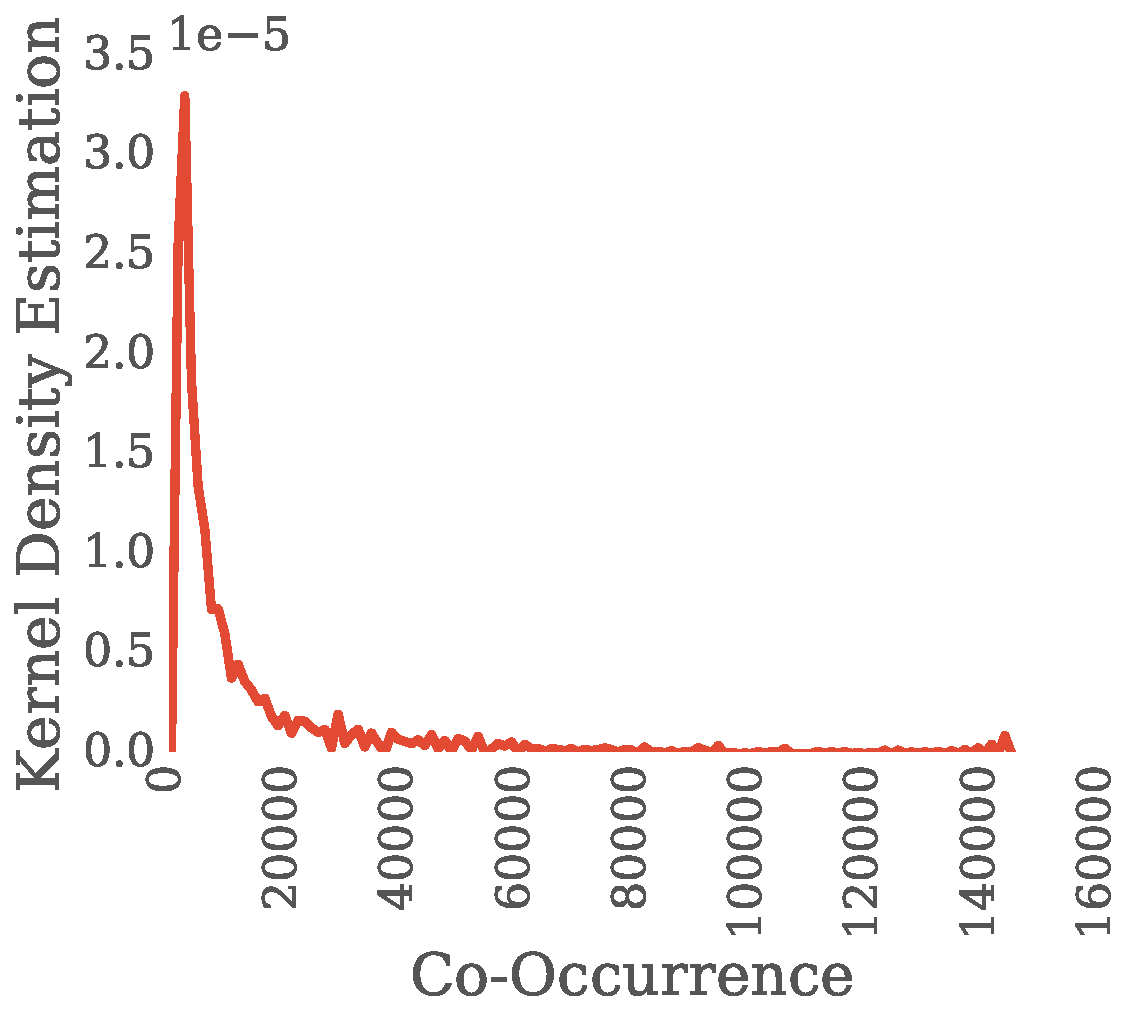
\includegraphics[width=0.23\textwidth]{kde_occurrencenetflix.pdf}~%
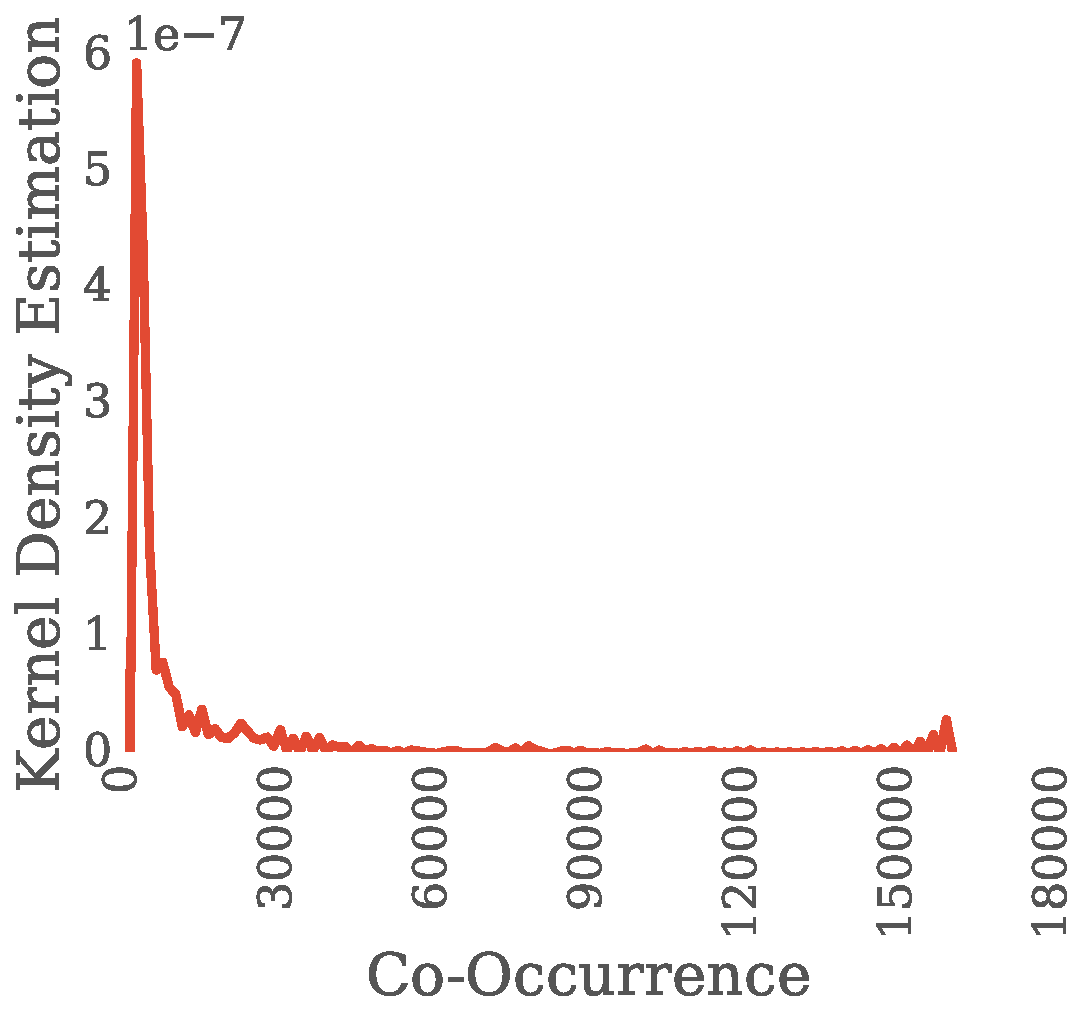
\includegraphics[width=0.22\textwidth]{kde_occurrenceymusic.pdf}
\caption{The Kernel Density Estimation of the item co-occurrence saturates in items that are infrequent. From left to right and top to bottom: Books, MovieLens, Netflix, Yahoo! Music.}
\label{fig:kde_occurrence}
\end{figure}

Our evaluation methodology is similar to \cite{koenigstein2013towards}. To generate the training and testing set we place most of the users in a training set and the rest of the users in the testing set. Then, we generate the pairs as described before. The number of training and testing pairs and the properties of the data sets can be seen in Table~\ref{tab:datasets}.
During testing the evaluation was performed over a sampled set of 200 items as in \cite{koenigstein2013towards} for all three metrics and solved ties arbitrary in the ranking except 
in case of MPR. % because the expected value of the cumulative frequency of surpassing items will be the same.

\begin{table}[t]
\caption[]{Data sets used in the experiments.}
\centerline{
\begin{tabular}{lrrrrr}\hline
\toprule
Data set       & Items  & Users  & Training & Testing\\
               &        &	 & pairs    & pairs \\
\midrule
Netflix        & 17,749  & 478,488 & 7,082,109  & 127,756 \\
MovieLens      & 3,683   & 6,040   & 670,220   & 15,425 \\
Yahoo!\ Music  & 433,903 & 497,881 & 27,629,731 & 351,344\\
Books      & 340,536 & 103,723 & 1,017,118  & 37,403 \\
\bottomrule
\end{tabular}
}
\label{tab:datasets}
\end{table}

In our experiments, all algorithms use the item frequencies of the training period as input parameters. However, it could be possible to keep the current frequencies up to date and recalculate the prediction of each algorithm on the fly.

\subsection{Experimental Results}

\newcommand\baslin[1]{#1}
\newcommand\bestal[1]{\textbf{#1}}

This section presents different experiments related to the size of the sample set, the modalities used (e.g. implicit, content), the performance on infrequent items and finally the overall performance. Table~\ref{tab:model_acronyms} explains the acronyms.

\begin{table}[t]
\caption[]{Model Acronyms}
\centerline{
\begin{tabular}{lrrrr}\hline
\toprule
      Acronym &  Description \\
\midrule
	FC & Model from Section~\ref{sect:FC} followed by similarity\\
	FD & Model from Section~\ref{sect:FD} followed by similarity\\
    FC content & FC with content similarity\\
    FD content & FD with content similarity\\
    FC multimodal & FC with content and collaborative similarity\\
\bottomrule
\end{tabular}
}
\label{tab:model_acronyms}
\end{table}


\subsubsection{Sample Set} 
The similarity graphs are defined via the set of items used as samples (Figs.~\ref{fig:pairwise}--~\ref{fig:multi}). To smooth the Fisher vector representation of sparse items we choose the most popular items in the training set as elements for the sample set. As we can see in Figures~\ref{fig:samples_recall}, ~\ref{fig:samples_dcg}, ~\ref{fig:samples_mpr}, recommendation quality saturates at a certain sample set size. Therefore we set the size of the sample set to $20$ for the remaining experiments. 

\begin{figure}[t]
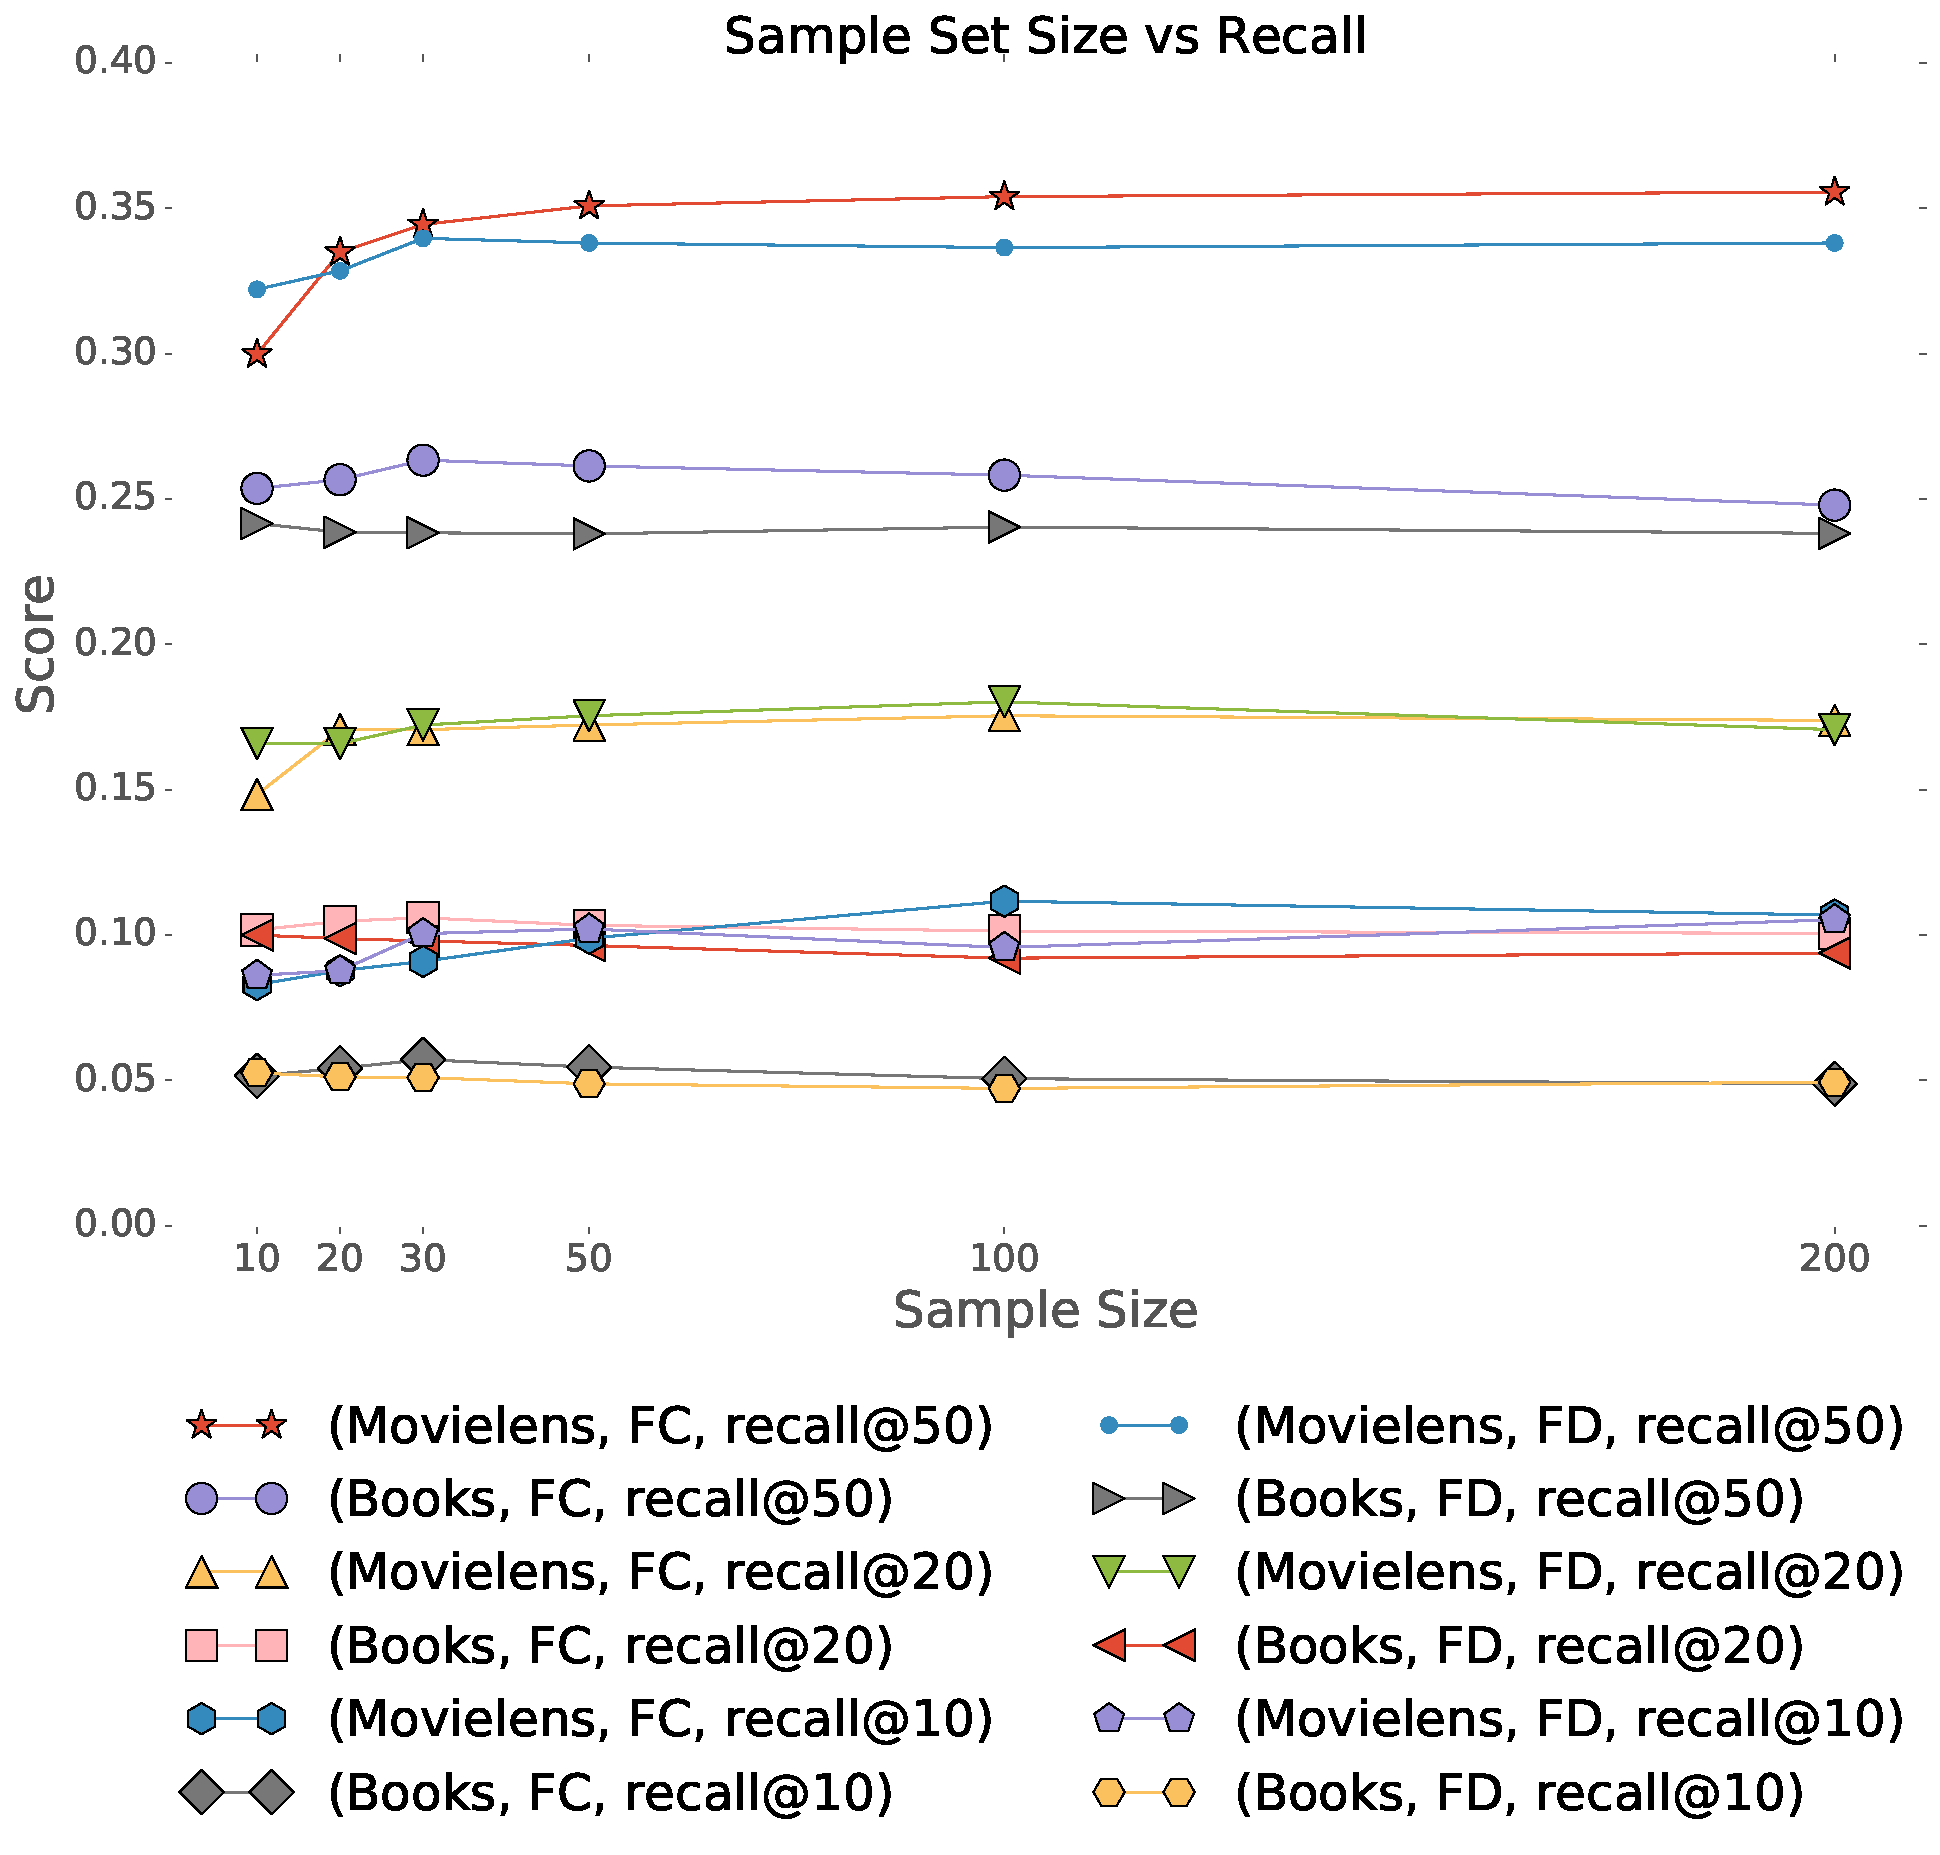
\includegraphics[width=0.5\textwidth]{reference_size_vs_Recall.pdf}
\caption[]{The sample set size improves Recall until it saturates at 50. In this example we use Jaccard similarity.}
\label{fig:samples_recall}
\end{figure}
\begin{figure}[t]
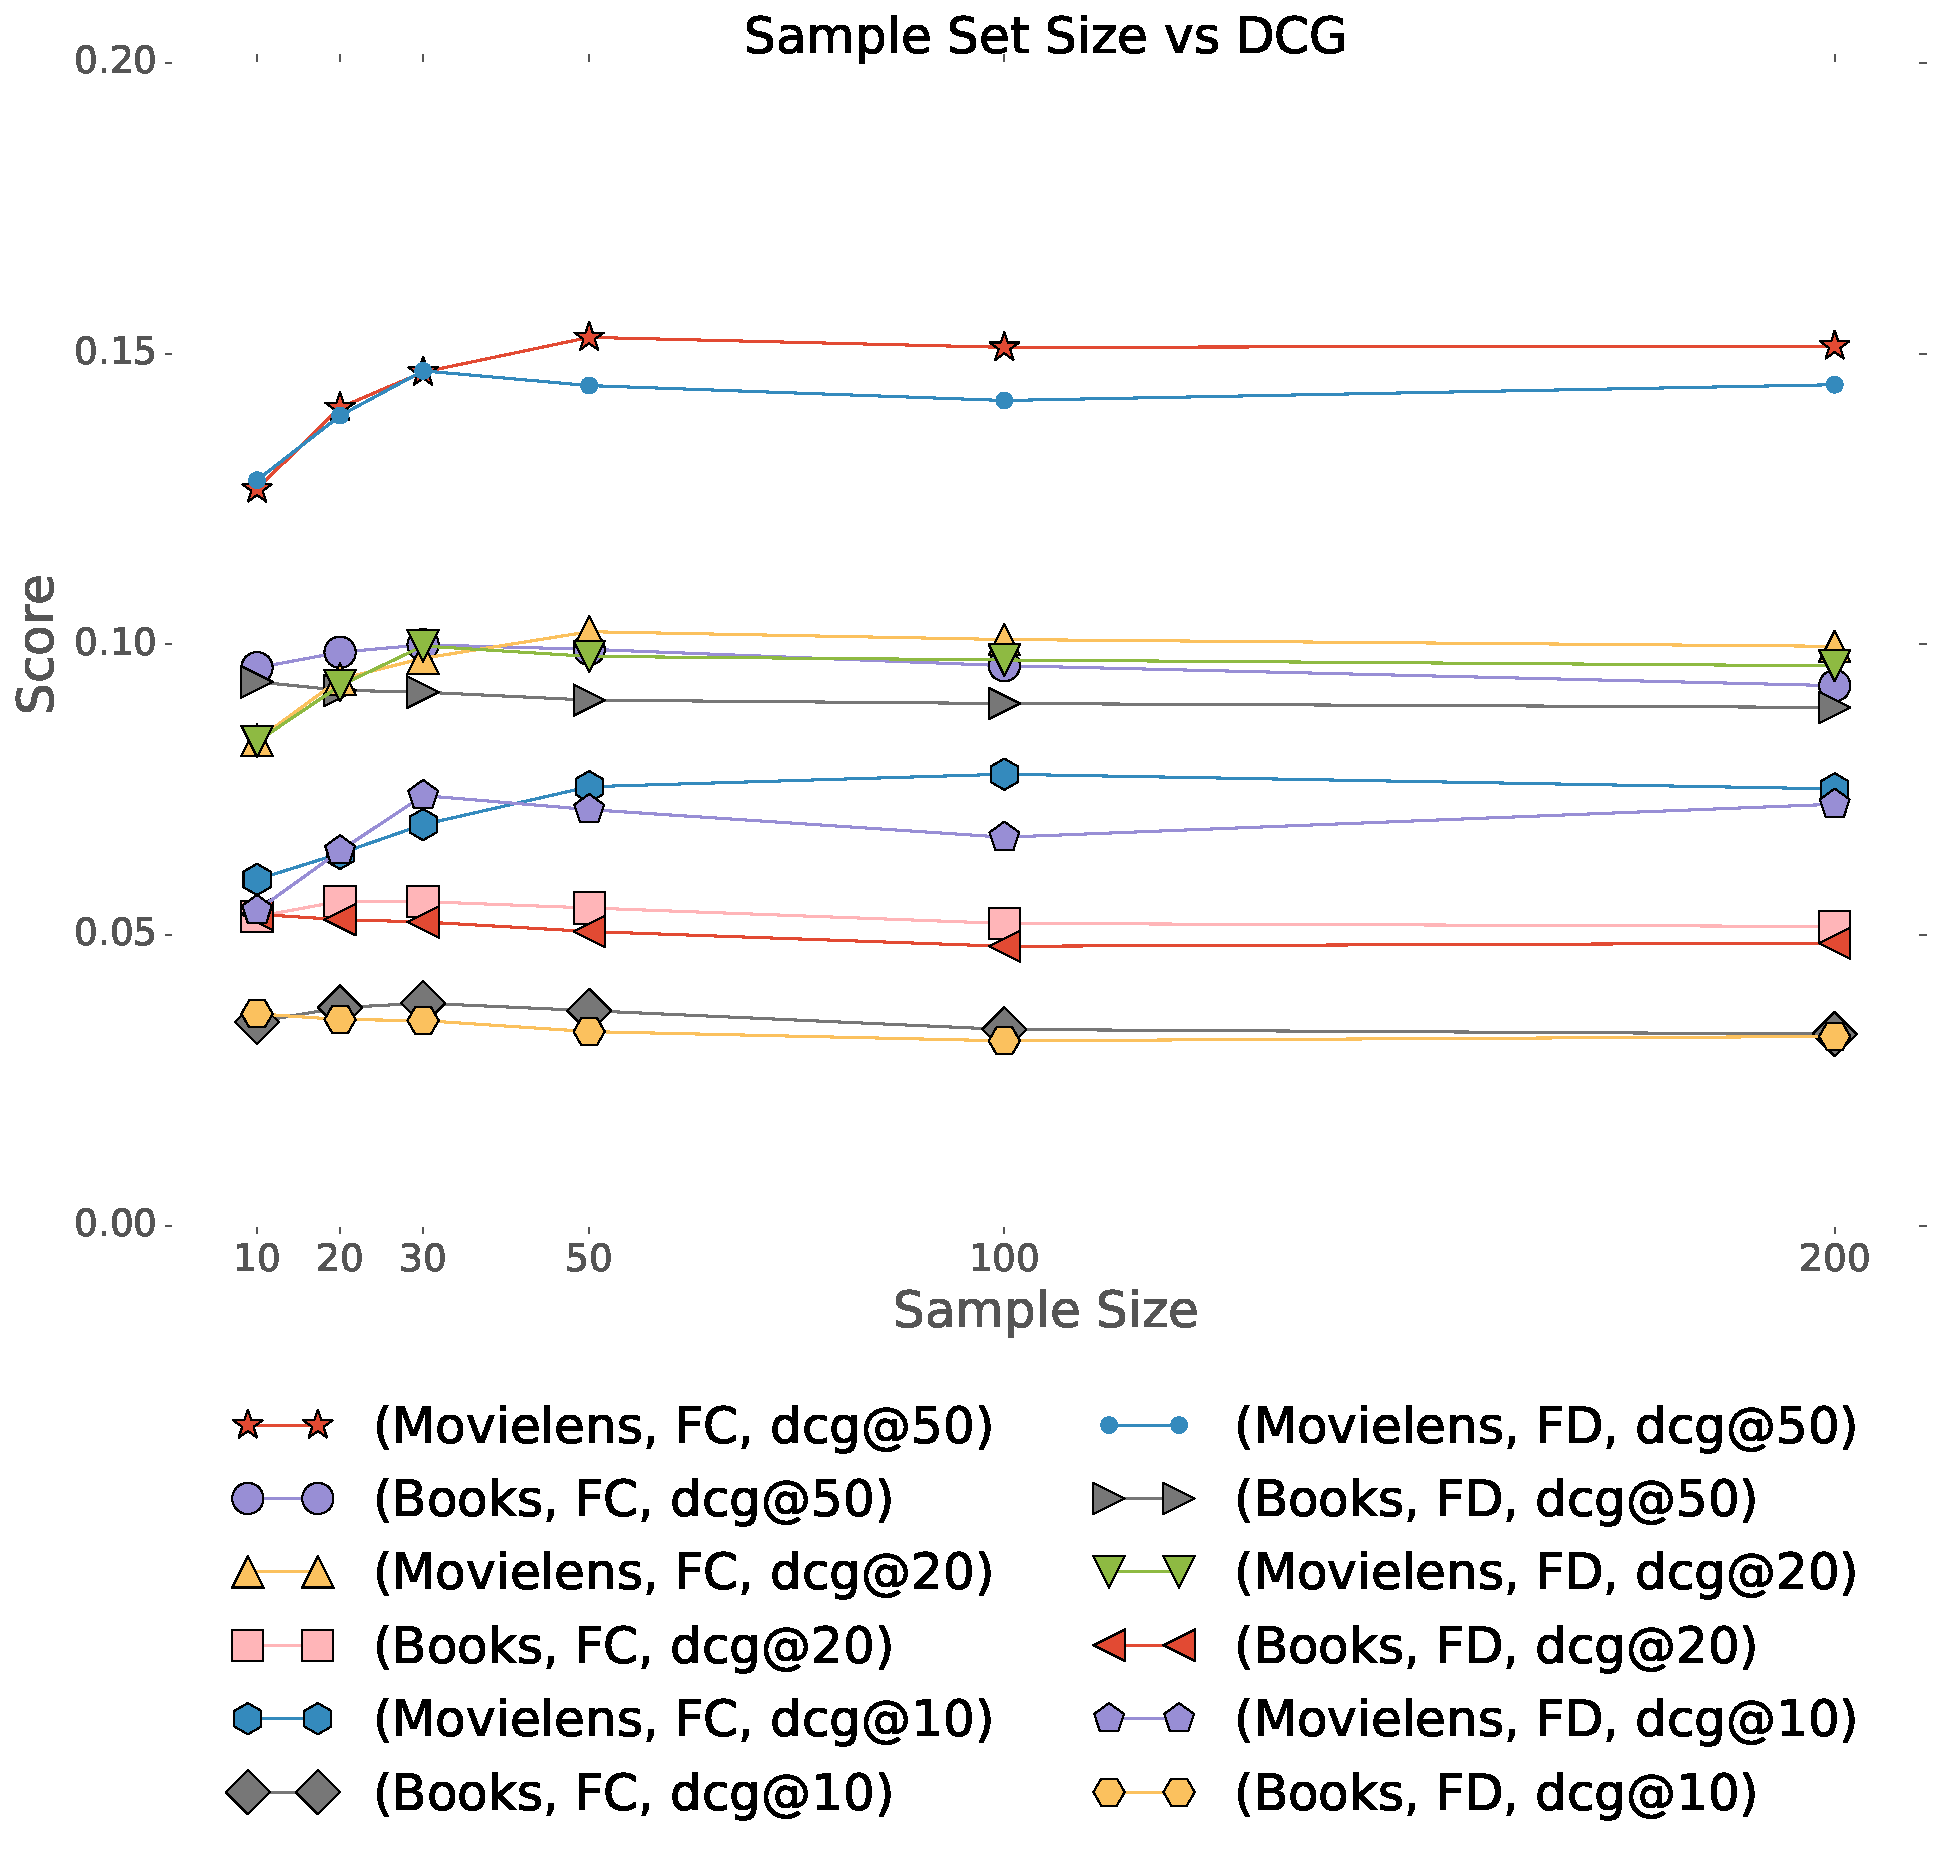
\includegraphics[width=0.5\textwidth]{reference_size_vs_DCG.pdf}
\caption[]{The sample set size improves DCG until it saturates at 50. In this example we use Jaccard similarity.}
\label{fig:samples_dcg}
\end{figure}
\begin{figure}[t]
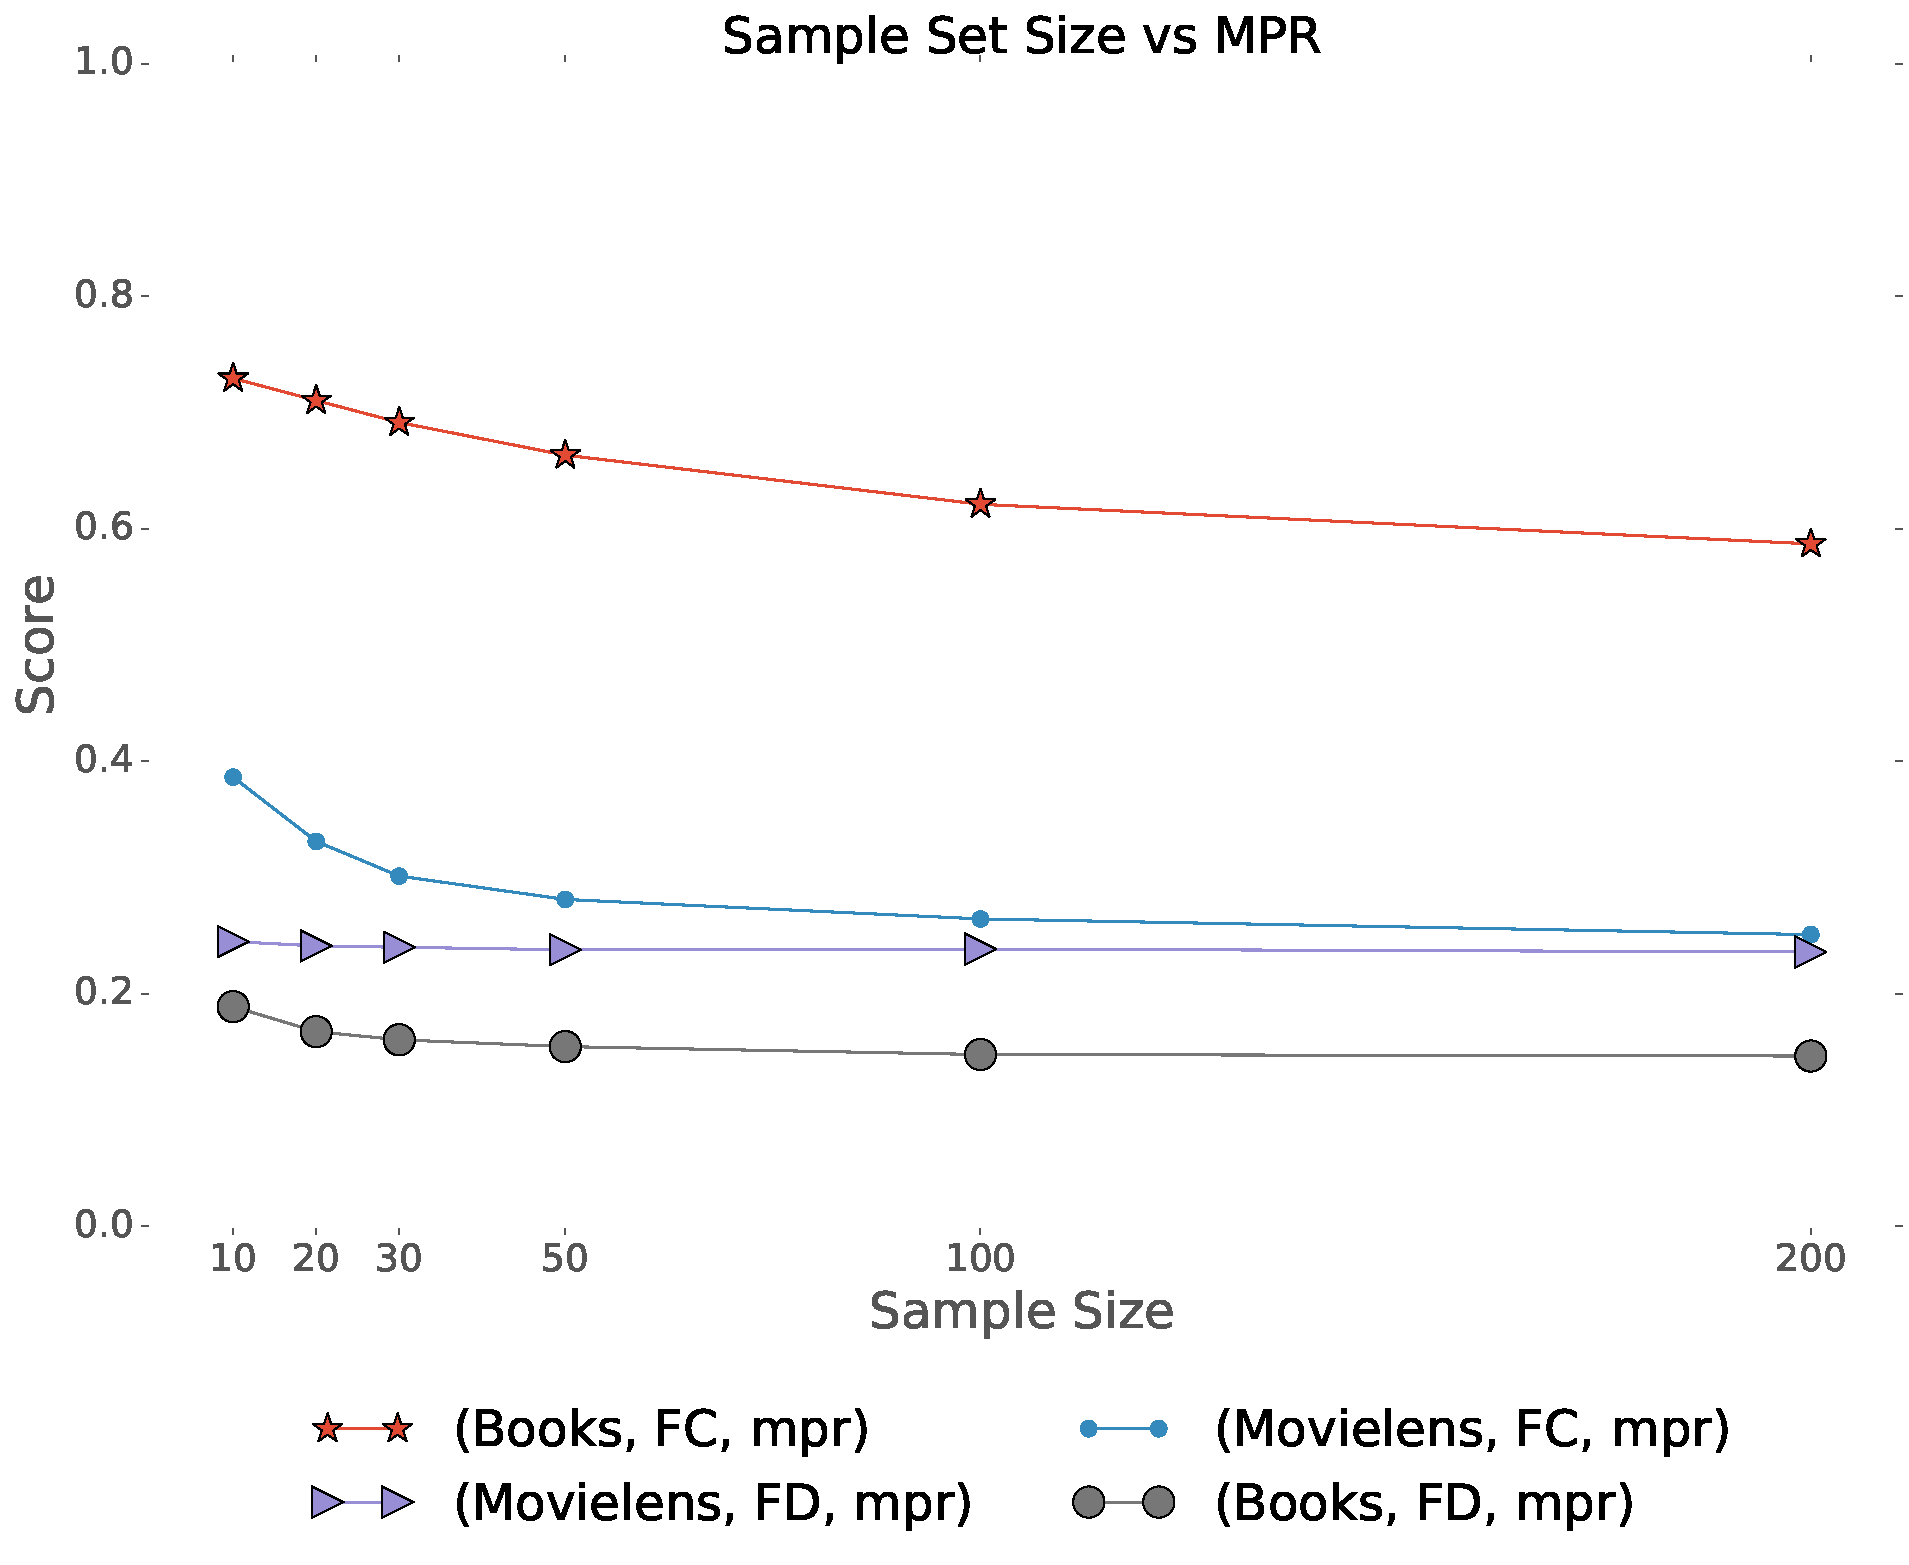
\includegraphics[width=0.5\textwidth]{reference_size_vs_MPR.pdf}
\caption[]{The sample set size improves MPR until it saturates at 50. In this example we use Jaccard similarity.}
\label{fig:samples_mpr}
\end{figure}

\subsubsection{Performance of Similarity Functions} 
Another relevant parameter of the similarity graphs is the choice of the similarity functions. Table~\ref{tab:exp_infreq_comb} presents the performance of the different similarity functions. Overall, Jaccard similarity is the best performing and we used it for the rest of our experiments.

\begin{table} 
\caption[]{Experiments with combination of collaborative filtering for the least frequent (25\%) conditional items of the MovieLens data.}
\centering
    \begin{tabular}{lccc}
& MPR & Recall@20 & DCG@20 \\ \hline
Cosine			& 0.4978		& 0.0988 		& 0.0553	\\ 
Jaccard			& 0.4978		& 0.0988		& 0.0547	\\ 
ECP			& 0.4976 		& 0.0940 		& \baslin{0.0601}	\\ 
EIR			& \baslin{0.3203}	& \baslin{0.1291} 	& 0.0344	\\ 
FC Cosine		& 0.3583		& 0.1020		& 0.0505	\\ 
FD Cosine		& 0.2849		& 0.1578		& 0.0860	\\ 
FC Jaccard		& 0.3354		& 0.1770 		& \bestal{0.1031}	\\ 
FD Jaccard		& \bestal{0.2415}	& \bestal{0.1866} 	& 0.1010\\ 
FC ECP			& 0.2504		& 0.0940		& 0.0444\\ 
FD ECP			& 0.4212		& 0.1626 		& 0.0856\\ 
FC EIR			& 0.4125		& 0.0861 		& 0.0434\\ 
FD EIR			& 0.4529		& 0.1068		& 0.0560\\ \hline

%FC + FD Jaccard		& 0.3606 		& 0.1196		& 0.0709	\\\hline

%FC JC + Cosine		& 0.327		& 0.1515 	& 0.0785	\\ 
%FC JC + Jaccard	& 0.327		& 0.1515		& 0.0785	\\ 
%FC JC	+ ECP		& 0.391		& 0.0893		& 0.0778	\\ 
%FC JC	+ EIR		& 0.3902 	& 0.1084		& 0.0557	\\ \hline 
%FD JC + Cosine		& 0.3026 	& 0.0749	 	& 0.0423	\\ 
%FD JC + Jaccard	& 0.3026 	& 0.0749 	& 0.0423	\\ 
%FD JC	+ ECP		& 0.2385 	& 0.161		& 0.0416	\\ 
%FD JC	+ EIR		& 0.2805 	& 0.1307		& 0.0394\\ \hline
    \end{tabular}
      \label{tab:exp_infreq_comb}
\end{table}

\subsubsection{Performance on Infrequent Items} 
One of the main challenges in the field of recommendation systems is the ``cold start'' problem, therefore we examine the performance in case of low item support. Figure~\ref{fig:supp_netf} shows the advantage of the Fisher methods for infrequent items.  As support increases, best results are reached by blending based on item support. If the current session ends with an item of high support, we may take a robust baseline recommender.  And if the support is lower, less than around 100, Fisher models can be used to compile the recommendation.

\begin{figure}
\centerline{
  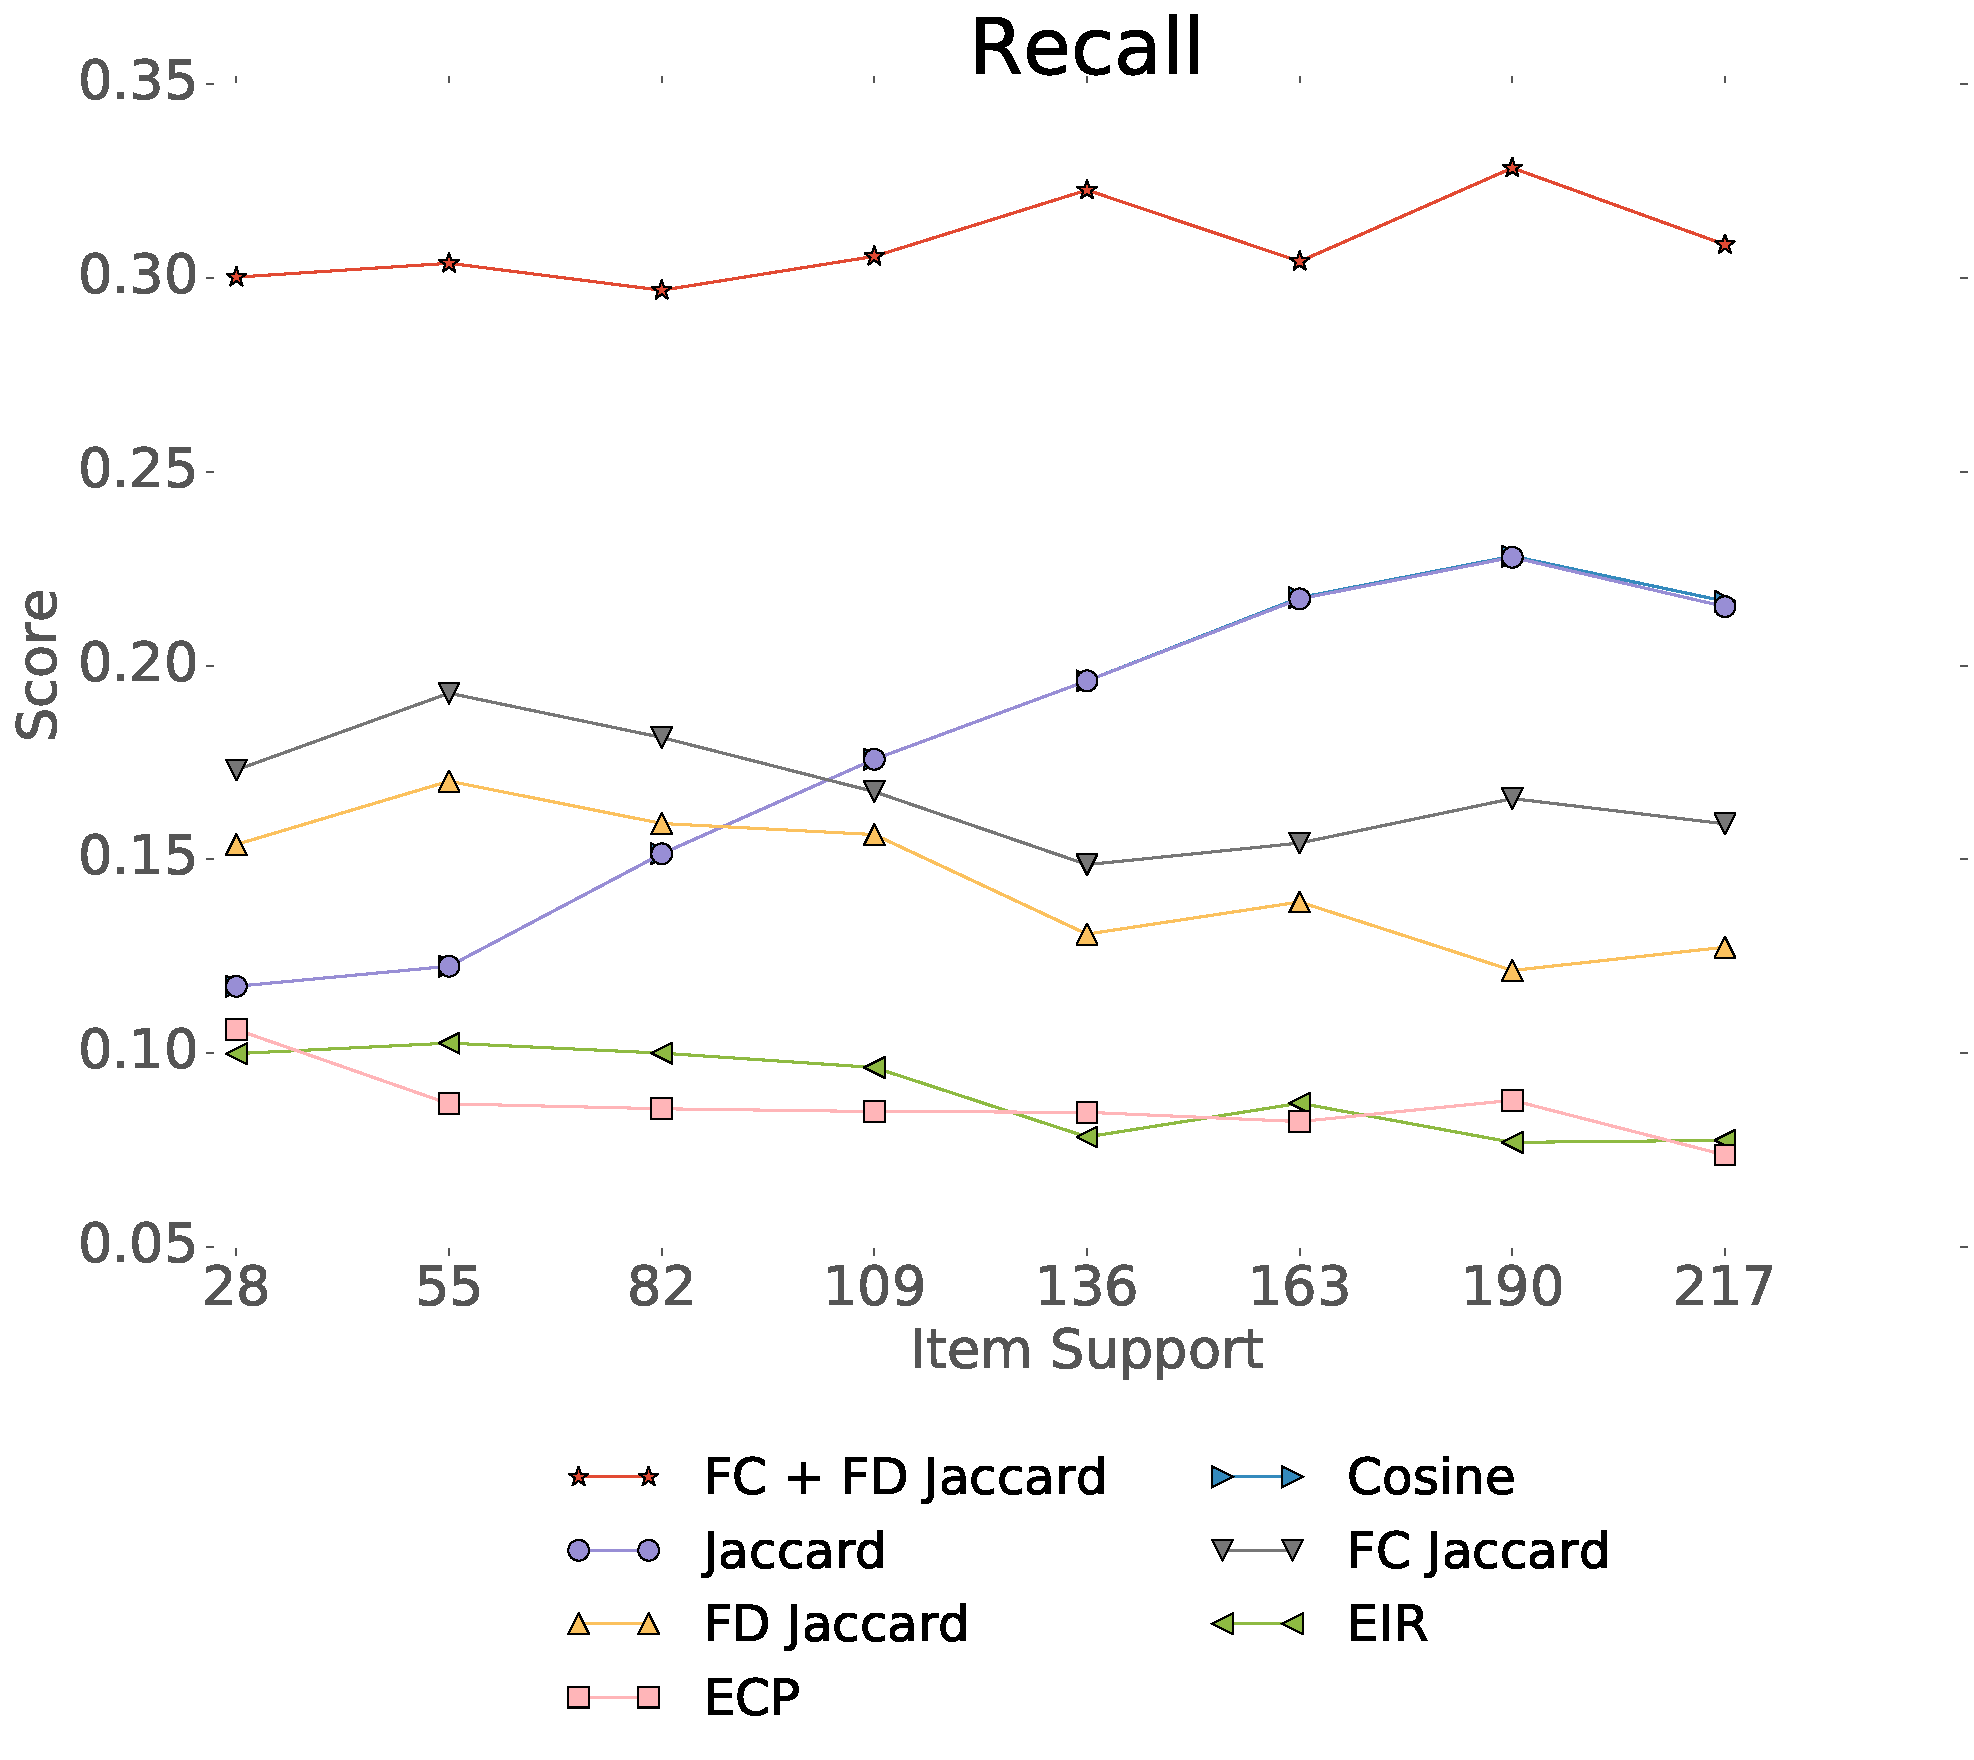
\includegraphics[width=0.5\textwidth]{nf_new.pdf}}
\caption[]{Recall@20 as the function of item support for the Netflix data set.
%FD + FC stands for the linear combination of the scores of FD and FD Jaccard.
}
\label{fig:supp_netf}
\end{figure}

In Fig.~\ref{fig:sparsity} we can see the item-to-item similarity values between the least frequent and between the most frequent items for different models. The feedback-based similarity may result arbitrary 
ranking for the least frequent items in comparison to the Fisher based similarity using the same modality. As expected the density of the content-based similarity models are more balanced. 

\begin{figure}
\centerline{
  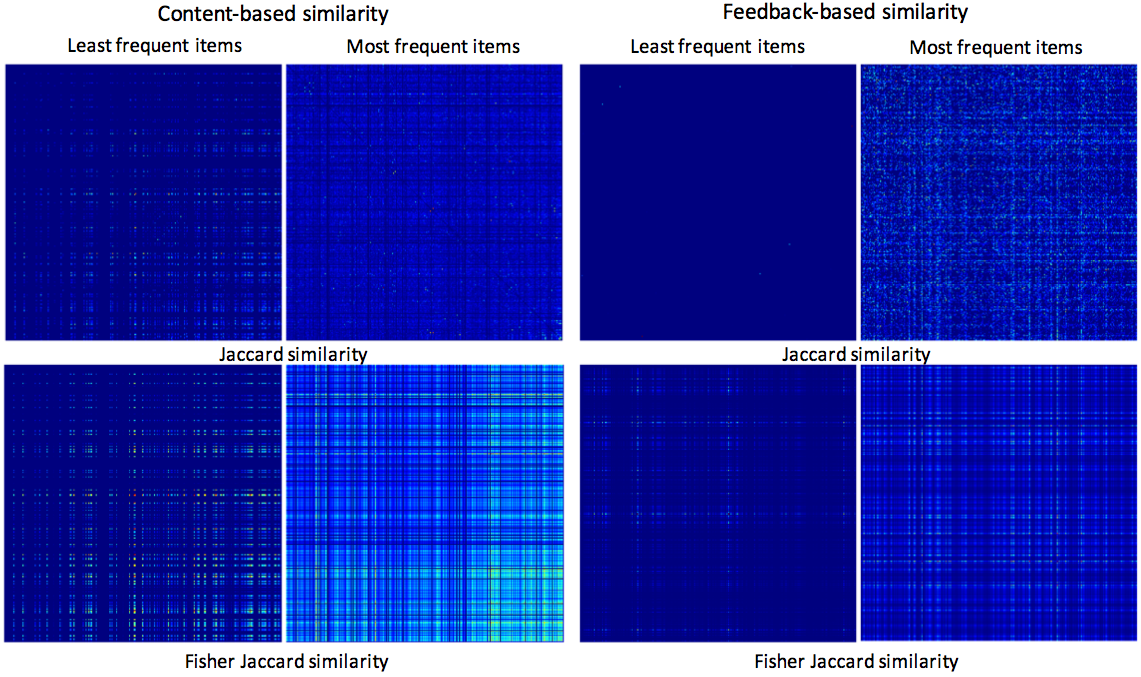
\includegraphics[scale=.21]{Sparsity.png}}
\caption[]{Density of different similarity measures between the least frequent items and between the most frequent items on MovieLens data set. Note we set the diagonal to zero to highlight non diagonal entries.}
\label{fig:sparsity}
\end{figure}

\subsubsection{Modalities: Implicit Feedback and Content} 
% Finally we turn to our content based and multimodal, mixed content and feedback recommendation experiments.
In Table~\ref{tab:exp_content} we show our experiments with DBPedia content as a modality on MovieLens. Due the complexity of the corresponding RDF graphs, we set the size of the sample set for both Fisher models to 10. 
The overall best performing model is the multimodal Fisher with Jaccard similarity, while every unimodal Fisher method outperform the baselines. 

\begin{table} 
\caption[]{Experiments on MovieLens with DBPedia content, all methods using Jaccard similarity.  
%FC and FD are the Fisher information methods of Sections~\ref{sect:FC} and~\ref{sect:FD} and multimodal uses the mix of both content and collaborative similarity.}
%JC and JS denote Jaccard and Jensen-Shannon, respectively, FC and FD are the Fisher information methods of Sections~\ref{sect:FC} and~\ref{sect:FD} and multimodal uses the mix of both content and collaborative similarity.
}
\centering
    \begin{tabular}{lcc}
			& Recall@20 	& DCG@20 \\ \hline
Collaborative baseline	& 0.139		& 0.057 \\
Content baseline      	& 0.131 	& 0.056 \\
%JS collaborative 	& 	& \\
FC content 		& 0.239 	& 0.108 \\
%FC JS content 		& 		& \\ 
FD content		& 0.214 	& 0.093 \\
%FD JS content		& 		& \\
FC multimodal    	& 0.275 	& 0.123 \\ \hline 
%FD JS multimodal 	& 		& \\\hline
    \end{tabular}
      \label{tab:exp_content}
\end{table}

Our experiments clearly show that the Fisher information based methods can blend different modalities such as content and feedback without the need of setting external parameters or applying learning for blending.  Note that for the results of Table~\ref{tab:exp_content}, we used the method of equation \eqref{eq:fk_multi} with no additional steps required for fusing the modalities.

\subsubsection{Summary of Performance vs Baselines} 
Tables~\ref{tab:exp_summary}--\ref{tab:exp_infreq_comb} present our results by relying on implicit feedback as our modality and compared to the baselines. The results are summarized and explained in the caption.

As expected, the choice of the distance function strongly affects the performance of the Fisher models. As seen in Table~\ref{tab:exp_infreq_comb}, the overall best performing distance measure is Jaccard for both types of Fisher models. 
The results in Table~\ref{tab:exp_summary} show that the linear combination of the standard normalized scores of the Fisher methods outperforms the best unimodal methods (Fisher with Jaccard) in case of the Netflix and the Books data sets, while for the MovieLens and Yahoo!\ Music data sets the Fisher distance with Jaccard performs best. 

\begin{table} 
  % \caption[]{Experimentation summary with the best performing collaborative baseline and new method names and performance metrics shown by filtering items at three different maximum frequency thresholds.  For most methods, there are (up to rounding errors) two best baseline and another two best new method candidates, except for Recall where a third method Cosine appears in the cell marked by a star ($*$).
  \caption[]{Summary of experiments results for the four datasets. The \textit{Max freq} are defined in the frequency quartile (Table~\ref{tab:datasets_quartiles}). For most methods, there are (up to rounding errors) two best baseline and two best Fisher models, except for Recall where a third method Cosine appears in the cell marked by a star ($*$). The best methods are usually FD Jaccard and FC + FD.
%The full experimentation tables are included in the supplementary material.
}
\centering
\begin{tabular}{rlrrrrr} \hline
  &\multicolumn{1}{p{2cm}}{\scriptsize{Best baseline\& new method}}
  &\multicolumn{1}{p{0.6cm}}{\scriptsize{Max freq}}
  &\multicolumn{1}{p{0.8cm}}{\scriptsize{Movie\-Lens}}
  &\multicolumn{1}{p{0.8cm}}{\scriptsize{Books}}
  &\multicolumn{1}{p{0.8cm}}{\scriptsize{Yahoo!\ Music}}
  &\multicolumn{1}{p{0.8cm}}{\scriptsize{Net\-flix}} \\ \hline 
         \multirow{7}{*}{{\rotatebox[origin=c]{90}{MPR}}}
& EIR            & 25\% &\baslin{0.33}&\baslin{0.48} &\baslin{0.24}&\baslin{0.34} \\
&                & 50\% &\baslin{0.35}&\baslin{0.48} &\baslin{0.25}&\baslin{0.35} \\
&                & 75\% &\baslin{0.36}&\baslin{0.47} &\baslin{0.25}&\baslin{0.38} \\ \cline{2-7}
& FD Jaccard     & 25\% &\bestal{0.24}&\bestal{0.24} &\bestal{0.06}&\bestal{0.31} \\
&                & 50\% &\bestal{0.26}&\bestal{0.24} &\bestal{0.06}&\bestal{0.32} \\
&                & \multirow{2}{*}{{75\%}}& &        &\bestal{0.08}&\bestal{0.34} \\
& FD + FC        &      &\bestal{0.34}&\bestal{0.25} &             &              \\ \hline
	\multirow{12}{*}{{\rotatebox[origin=c]{90}{Recall@20}}}
& Jaccard        & 25\% &             &              &             &\baslin{0.13} \\
&                & 50\% &             &              &             &\baslin{0.18} \\
&                & 75\% &\baslin{0.12$^*$}&          &             &\baslin{0.20} \\
& EIR            & 25\% &\baslin{0.12}&\baslin{0.10} &\baslin{0.13}& \\ 
&                & 50\% &\baslin{0.11}&\baslin{0.10} &\baslin{0.11}& \\
&                & 75\% &             &\baslin{0.10} &\baslin{0.12}& \\ \cline{2-7}
& FD Jaccard     & 25\% &\bestal{0.18}&              &\bestal{0.23}& \\
&                & 50\% &\bestal{0.19}&              &\bestal{0.23}& \\
&                & 75\% &\bestal{0.14}&              &\bestal{0.20}& \\
&  FC + FD       & 25\% &             &\bestal{0.14} &             &\bestal{0.30} \\
&                & 50\% &             &\bestal{0.14} &             &\bestal{0.30} \\
&                & 75\% &             &\bestal{0.13} &             &\bestal{0.31} \\ \hline
	     \multirow{12}{*}{{\rotatebox[origin=c]{90}{DCG@20}}}
& ECP            & 25\% &\baslin{0.05}&             &             &        \\
&                & 50\% &\baslin{0.05}&             &             &        \\
&                & 75\% &\baslin{0.05}&             &             &        \\
& EIR            & 25\% &             &\baslin{0.06}&\baslin{0.05}& \baslin{0.12} \\
&                & 50\% &             &\baslin{0.06}&\baslin{0.05}& \baslin{0.12} \\
&                & 75\% &             &\baslin{0.06}&\baslin{0.05}& \baslin{0.12} \\  \cline{2-7}
& FD Jaccard     & 25\% &\bestal{0.10}&             &\bestal{0.11}&        \\
&                & 50\% &\bestal{0.11}&             &\bestal{0.11}&        \\
&                & 75\% &\bestal{0.08}&             &\bestal{0.10}&        \\
&  FC + FD       & 25\% &             &\bestal{0.08}&             &\bestal{0.17} \\ 
&                & 50\% &             &\bestal{0.08}&             &\bestal{0.17} \\ 
&                & 75\% &             &\bestal{0.08}&             &\bestal{0.17} \\ \hline
\end{tabular}
      \label{tab:exp_summary}
\end{table}

\section{Limitations and Future Work}

Recommending infrequent item-to-item transitions without personalized user history is a challenging problem. Our experiments were limited by the publicly available data sets. Future work could be to experiment with real sessions, especially within a short period of time, e.g. news recommendation. In addition, we constrained our similarity graphs for simple item-to-item transitions, defining the next item in the ``random walk'' depending only on the last seen item. To find out the limitation of this hypothesis we intend to expand the generative model to utilize the previous items in a session. 

We consider our results for simple, non-personalized item-to-item recommendation as first step towards demonstrating the power of the method. As a key feature, we are able to fuse different modalities including collaborative filtering, content and side information, without the need for learning weight parameters or using wrapper methods. In the future, we plan to extend our methods to personalized recommendation settings and refine the underlying similarity measures with complex models (e.g. neural networks \cite{deep_learning_recsys}). 

\section{Conclusions}

In this paper, we considered the session based item-to-item recommendation task, in which the recommender system has no personalized knowledge of the user beyond the last items visited in the current user session.
We proposed Fisher information based global item-item similarity models for this task.
We reached significant improvement over existing methods in case of infrequent item-to-item transitions by experimenting with a variety of data sets as well as evaluation metrics. In particular, by making the best effort to 
reproduce the experiments of \cite{koenigstein2013towards}, we showed that our method is superior in all aspects, even if we only use the implicit item ratings for recommendation.

We made our experiments fully reproducible by releasing the source code of not just the algorithm, but also the preprocessing steps taken over the standard 
experimentation data sets used in our measurements.

%\section{Acknowledgments}
%The publication was supported by the PIAC\_13-1-2013-0205 project of the Research and Technology Innovation Fund, by the Momentum Grant of the Hungarian Academy of Sciences and by the Mexican Postgraduate Scholarship of the Mexican National Council for Science and Technology (CONACYT). 
